\setcounter{chapter}{3}

\chapter{Categorial Explanatory Variables}


{\small \textit{Chapter Preview}. \textit{Categorical variables}
allow us to group observations into distinct categories. This
chapter shows how to incorporate categorical variables into
regression functions using binary variables, thus considerably
widening the scope of potential applications for regression
analysis. Statistical inference for several coefficients is
introduced in this chapter to allow analysts to make decisions about
categorical variables (as well as other important applications).
Categorical explanatory variables also provide the basis of
\textit{ANOVA} models, representations which are equivalent to
regression in some circumstances that permit easier interpretation
and analysis.}

\section{The Role of Binary Variables}

\textit{Categorical variables} provide labels for observations to
denote membership in distinct groups, or categories. A binary
variable is a special case of a categorical variable. To illustrate,
a binary variable may tell us whether or not someone has health
insurance. A categorical variable could tell us whether someone has
(i) private individual health insurance, (ii) private group
insurance, (iii) public insurance or (iv) no health insurance.

For categorical variables, there may or may not be an ordering of
the groups. For health insurance, it is difficult to say which is
``larger,'' private individual versus public health insurance (such
as Medicare). However, for education, we may group individuals from
a dataset into ``low,'' ``intermediate'' and ``high'' years of
education. In this case, there is an ordering among groups; this
ordering may or may not provide information about the dependent
variable. \textit{Factor} is another term used for a (unordered)
categorical explanatory variable.

For ordered categorical variables, analysts typically assign a
numerical score to each outcome of the variable and treat it as if
it were a continuous variable. For example, if we had three levels
of education, we might employ ranks and use
\begin{equation*}
\textrm{EDUCATION} = \left\{ \begin{array}{cl}
        1           & \textrm{for low education} \\
        2           & \textrm{for intermediate education} \\
        3           & \textrm{for high education} \\
\end{array} \right. .
\end{equation*}
Another alternative would be to use numerical scores that
approximate the underlying value of the category. For example, we
might use
\begin{equation*}
\textrm{EDUCATION} = \left\{ \begin{array}{cl}
        6           & \textrm{for low education} \\
        10           & \textrm{for intermediate education} \\
        14           & \textrm{for high education} \\
\end{array} \right. .
\end{equation*}
This gives the approximate number of years of schooling that
individuals in each category receive.

The assignment of numerical scores and treating the variable as
continuous has important implications for the regression modeling
interpretation. Recall that the regression coefficient is the
marginal change in the expected response so that the $\beta$ for
education assesses the increase in E $y$ per unit change in
EDUCATION. If we record EDUCATION as a rank, then this assumes that
the increase in E $y$ is the same as moving from EDUCATION=1 to
EDUCATION=2 (from low to intermediate) as moving from EDUCATION=2 to
EDUCATION=3 (from intermediate to high). This is an assumption that
the analyst makes with this coding of EDUCATION that may or may not
be valid in the application.

Because of this interpretation of coefficients, analysts rarely use
ranks to summarize \emph{unordered} categorical variables. The most
direct way of handling categorical variables in regression is
through the use of binary variables. A categorical variable with $c$
levels can be represented using $c$ binary variables, one for each
category. For example, suppose that for we were not sure of the
direction of the education effect and so decide to treat it as an
unordered categorical variable. Then, we could code $c$=3 binary
variables: (1) a variable to indicate low education, (2) one to
indicate intermediate education and (3) one to indicate high
education. These binary variables are often known as \emph{dummy
variables}. In regression analysis with an intercept term, we use
only $c$-1 of these binary variables. The remaining variable enters
implicitly through the intercept term. By identifying a variable as
a factor, most statistical software packages will automatically
create binary variables for you.

Through the use of binary variables, we do not make use of the
ordering of categories within a factor. Because no assumption is
made regarding the ordering of the categories, for the model fit it
does not matter which variable is dropped with regard to the fit of
the model. However, it does matter for the interpretation of the
regression coefficients. Consider the following example.

\linejed

\bigskip
\textbf{Example: Term Life Insurance - Continued.} We now return to
the marital status of respondents from the Survey of Consumer
Finances (SCF). Recall that marital status is not measured
continuously but rather takes on values that falls into distinct
groups that we treat as unordered. In Chapter 3, we grouped survey
respondents according to whether or not they are single, defined to
be separated, divorced, widowed or never married, and are not
married nor living with a partner. We now supplement this by
considering the categorical variable, MARSTAT, that is the marital
status of the survey respondent. This may be:
\begin{itemize}
 \item 1, for married
 \item 2, for living with partner
 \item 0, for other (SCF breaks this category into
 separated, divorced, widowed, never married and inapplicable, for
 persons age 17 or less or no further persons)
 \end{itemize}

As before, the dependent variable is $y$ = LNFACE, the amount that
the company will pay in the event of the death of the named insured
(in logarithmic dollars). Table \ref{T4:MaritalSumStats} summarizes
the dependent variable by level of the categorial variable. This
table shows that the marital status ``married'' is the most
prevalent in the sample and that those married choose to have the
most life insurance coverage. Figure \ref{F4:BoxFACEMARSTAT} gives a
more complete picture of the distribution of LNFACE for each of the
three types of marital status. The table and figure also suggests
that those living together have less life insurance coverage than
the other two categories.


\begin{table}[h] \caption{\label{T4:MaritalSumStats} Summary
Statistics of Logarithmic Face By Marital Status}
\begin{tabular}{lcccc}
\hline
& MARSTAT & Number & Mean & Standard \\
&  &  &  & deviation \\ \hline
Other           & 0 & 47 & 11.01 & 1.455 \\
Married         & 1 & 155 & 12.50 & 1.794 \\
Living together & 2 & 10 & 10.51 & 1.314 \\ \hline
Total           &   & 212 & 12.07 & 1.840 \\
 \hline
\end{tabular}
\end{table}


\begin{figure}[htp]
  \begin{center}
    \includegraphics[width=1\textwidth,angle=270,scale=0.5]{Chapter4/Fig41Boxplot1.ps}
       \caption{\label{F4:BoxFACEMARSTAT} \small  Box Plots of Logarithmic Face, by Level of Marital Status.}
  \end{center}
\end{figure}

Are the continuous and categorical variables jointly important
determinants of response? To answer this, a regression was run using
LNFACE as the response, three continuous variables and two binary
variables of the marital status. Recall that our three continuous
variables are:  LNINCOME, logarithmic annual income, the number of
years of EDUCATION of the survey respondent and the number of
household members, NUMHH.

Define MAR0 to be the binary variable that is one if MARSTAT=0 and
zero otherwise. Similarly, define MAR1 and MAR2 to be binary
variables that indicate MARSTAT=1 and MARSTAT=2, respectively. There
is a perfect linear dependency among these three binary variables in
that $MAR0 + MAR1 + MAR2 = 1$ for any survey respondent. However,
there is \emph{not} a perfect dependency among any two of the three.
It turns out that $Cor(MAR0,MAR1) = -0.88$, $Cor(MAR0,MAR2) =-0.12$
and $Cor(MAR1,MAR2) = -0.37$.

A regression equation was run using LNINCOME, EDUCATION, NUMHH, MAR0
and MAR1 as explanatory variables. The fitted regression equation
turns out to be
   \begin{eqnarray*}
\widehat{y} &=& 4.915 + 0.308 LNINCOME +0.214 EDUCATION + 0.253
NUMHH \\
 & & ~~ -0.518 MAR0 -1.222 MAR2
\end{eqnarray*}

\begin{itemize}
\item If you are married, then $MAR0=0$, $MAR1=1$ and $MAR2=0$, and
   \begin{eqnarray*}
\widehat{y} &=& 4.915 + 0.308 LNINCOME +0.214 EDUCATION + 0.253
NUMHH
\end{eqnarray*}
\item If living together, then $MAR0=0$, $MAR1=0$ and $MAR2=1$, and
   \begin{eqnarray*}
\widehat{y} &=& 4.915 + 0.308 LNINCOME +0.214 EDUCATION + 0.253
NUMHH -1.222
\end{eqnarray*}
\item The difference in these two equations is $-1.222.$
\end{itemize}

Interpret the regression coefficient associated with $MAR2$ to be
the difference in fitted value for someone living together, compared
to a similar person who is married (the omitted category).


Similarly, interpret -0.518 to be the difference between the
``other'' category and the married category.

$-0.518 - (-1.222) =0.704$ is the difference between the other and
the living together category.






  \begin{itemize}
   \item Note that $MAR0 + MAR1 + MAR2 = 1$ - there is a $perfect$
   linear dependency among the three.
   \item
   \item Any two out of the three produce the same model in terms of
   goodness of fit
   \end{itemize}



 \begin{table}
 \scalefont{0.9}
\caption{Term Life with Marital Status ANOVA Table}
\begin{tabular}{lrrr}
 \hline Source
& Sum of Squares & $df$ & Mean Square \\ \hline

Regression & 237.78 & 5 &   47.56 \\
Error      & 476.74 & 206 &  2.31 \\
Total      & 714.52 & 211 &   \\ \hline
\end{tabular}

Residual standard error $s= 1.521$, $R^2 = 33.3\%$, $R_a^2 = 31.7\%$
\scalefont{1.1111}
\end{table}

\begin{table}
\scalefont{0.9} \caption{ Term Life Regression Coefficients}
\begin{tabular}{l|rr|rr|rr}
 \hline
 & \multicolumn{2}{c|}{Model 1}& \multicolumn{2}{c|}{Model 2}& \multicolumn{2}{c}{Model 3}\\
 \hline
 Explanatory & Coefficient & $t$-ratio & Coefficient & $t$-ratio& Coefficient &
 $t$-ratio\\
 Variable &&&&&&\\ \hline
LNINCOME & 0.308 & 3.40 & 0.308 & 3.40 & 0.308 & 3.40 \\
EDUCATION &0.214 & 4.61 &0.214 & 4.61&0.214 & 4.61 \\
NUMHH     & 0.253 & 2.97 & 0.253 & 2.97 & 0.253 & 2.97 \\\hline
Intercept & 3.693& 3.40& 4.915 & 4.58  & 4.397 & 4.50\\
MAR0    &  0.703 &  1.31 &-0.518& -1.71& &\\

MAR1 &  1.222 &   2.41 &  & &0.518 &1.71\\
MAR2 & & & -1.222 & -2.41 & 0.703& -1.31\\
 \hline
\end{tabular}
\scalefont{1.1111}
\end{table}

\linejed

\textbf{Example: How does Cost-Sharing in Insurance Plans affect
Expenditures in Healthcare?} In one of many studies that resulted
from the Rand Health Insurance Experiment (HIE) introduced in
Section 1.5, Keeler and Rolph (1988) investigated the effects of
cost-sharing in insurance plans. For this study, 14 health insurance
plans were grouped by the co-insurance rate (the percentage paid on
out-of-pocket expenditures that varied by 0, 25, 50 and 95\%). One
of the 95\% plans limited annual out-of-pocket outpatient
expenditures to \$150 per person (\$450 per family), providing in
effect an individual outpatient deductible. This plan was analyzed
as a separate group so that there were $c=5$ categories of insurance
plans. In most insurance studies, individuals choose insurance plans
making it difficult to assess cost-sharing effects because of
adverse selection. Adverse selection can arise because individuals
in poor chronic health are more likely to choose plans with less
cost sharing, thus giving the appearance that less coverage leads to
greater expenditures. In the Rand HIE, individuals were randomly
assigned to plans, thus removing this potential source of bias.

Keeler and Rolph (1988) organized an individual's expenditures into
episodes of treatment; each episode contains spending associated
with a given bout of illness, chronic condition or procedure.
Episodes were classified as hospital, dental or outpatient; this
classification was based primarily on diagnoses, not by location of
services. Thus, for example, outpatient services preceding or
following a hospitalization, as well as related drugs and tests,
were included as part of a hospital episode.

For simplicity, here we report only results for hospital episodes.
Although families were randomly assigned to plans, Keeler and Rolph
(1988) used regression methods to control for participant attributes
and isolate the effects of plan cost-sharing. Table
\ref{T4:RandHIECoefficients} summarizes the regression coefficients,
based on a sample of $n=1,967$ episode expenditures. In this
regression, logarithmic expenditure was the dependent variable.

The cost-sharing categorical variable was decomposed into five
binary variables so that no functional form was imposed on the
response to insurance. These variables are ``Co-ins25,''
``Co-ins50,'' and ``Co-ins95,'' for coinsurance rates 25, 50 and
95\%, respectively, and ``Indiv Deductible'' for the plan with
individual deductibles. The omitted variable is the free insurance
plan with 0\% coinsurance. The HIE was conducted in six cities; a
categorical variable to control for the location was represented
with five binary variables, Dayton, Fitchburg, Franklin, Charleston
and Georgetown, with Seattle being the omitted variable. A
categorical factor with $c=6$ levels was used for age and sex;
binary variables in the model consisted of ``Age 0-2,'' ``Age 3-5,''
``Age 6-17,'' ``Woman age 18-65,'' and ``Man age 46-65,'' the
omitted category was ``Man age 18-45.'' Other control variables
included a health status scale, socioeconomic status, number of
medical visits in the year prior to the experiment on a logarithmic
scale and race.

Table \ref{T4:RandHIECoefficients} summarizes the effects of the
variables. As noted by Keeler and Rolph, there were large
differences by site and age although the regression only served to
summarize $R^2=11\%$ of the variability. For the cost-sharing
variables, only ``Co-ins95'' was statistically significant, and this
only at the 5\% level, not the 1\% level.

The paper of Keeler and Rolph (1988) examines other types of episode
expenditures, as well as the frequency of expenditures. They
conclude that cost-sharing of health insurance plans has little
effect on the amount of expenditures per episode although there are
important differences in the frequency of episodes. This is because
an episode of treatment is composed of two decisions. The amount of
treatment is made jointly between the patient and the physician and
is largely unaffected by the type of health insurance plan. The
decision to seek health care treatment is made by the patient; this
decision-making process is more susceptible to economic incentives
in cost-sharing aspects of health insurance plans.


\begin{table}[h]
\caption{\label{T4:RandHIECoefficients} Coefficients of Episode
Expenditures from the Rand HIE}
\begin{tabular}{lr|lr}
   \hline
  Variable & Regression &   Variable & Regression \\
           & Coefficient &           & Coefficient \\
\hline
    Intercept &       7.95~ &            &            \\
    Dayton &       0.13* &    Co-ins25 &       0.07~~ \\
 Fitchburg &       0.12~ &    Co-ins50 &       0.02~~ \\
  Franklin &      -0.01~ &    Co-ins95 &      -0.13*~ \\
Charleston &       0.20* &    Indiv Deductible &      -0.03~~ \\
Georgetown &      -0.18* &            &            \\
           &            &            &            \\
Health scale &     -0.02* &    Age 0-2 &      -0.63** \\
Socioeconomic status &  0.03~ &    Age 3-5 &      -0.64** \\
Medical visits &      -0.03~ &   Age 6-17 &      -0.30** \\
Examination &      -0.10* & Woman age 18-65 &       0.11~~ \\
     Black &       0.14* & Man age 46-65 &       0.26~~ \\
 \hline
\multicolumn{4}{l}{Note: * significant at 5\%, ** significant at 1\%} \\
     \multicolumn{4}{l}{\textit{Source}: Keeler and Rolph (1988)} \\
      \hline
\end{tabular}
\end{table}


\linejed


\section{Statistical Inference for Several Coefficients}

In many applications, it is useful to examine several regression
coefficients at the same time. For example, we have already seen the
regression function in equation (3.5) expressed as a linear
combination of regression coefficients. As another example, when
assessing the effect of a categorical variable with $c$ levels, we
need to say something jointly about the $c-1$ binary variables that
enter the regression equation. To do this, Section 4.2.1 introduces
the idea of \emph{sets} of regression coefficients using matrix
algebra. Section 4.2.2 shows applications in the context of
hypothesis testing and Section 4.2.3 presents other inference
applications.


\subsection{Sets of Regression Coefficients}

Recall that our regression coefficients are specified by
$\boldsymbol \beta =\left( \beta_0, \beta_1, \ldots,\beta_k \right)
^{\prime },$ a $(k+1)\times 1$ vector. It will be convenient to
express linear combinations of the regression coefficients using the
notation $\mathbf{C} \boldsymbol \beta,$ where \textbf{C} is a
$p\times (k+1)$ matrix that is user-specified (depending on the
application). To demonstrate the broad variety of applications in
which sets of regression coefficients can be used, we now present a
series of special cases.

Some applications involve estimating $\mathbf{C} \boldsymbol \beta$.
Others involve testing whether $\mathbf{C} \boldsymbol \beta$ equals
a specific known value (denoted as \textbf{d}). We call
$H_0:\mathbf{C \boldsymbol \beta =d}$ the \emph{general linear
hypothesis}.

\textbf{Special Case 1 - One Regression Coefficient}. In Section
3.4, we investigated the importance of a single coefficient, say
$\beta_j.$ We may express this coefficient as $\mathbf{C}
\boldsymbol \beta$ by choosing $p=1$ and \textbf{C} to be a $1\times
(k+1$) vector with a one in the $(j+1)st$ column and zeros
otherwise. These choices result in
\begin{equation*}
\mathbf{C \boldsymbol \beta =}\left( 0~...~0~1~0~...~0\right) \left(
\begin{array}{c}
\beta_0 \\
\vdots  \\
\beta_k%
\end{array}
\right) =\beta_j.
\end{equation*}

\textbf{Special Case 2 - Regression Function}. Here, we choose $p=1$
and \textbf{C} to be a $1\times (k+1$) vector representing the
transpose of a set of explanatory variables. These choices result in

\begin{equation*}
\mathbf{C \boldsymbol \beta =}\left(x_0,x_1, \ldots, x_k \right)
\left(
\begin{array}{c}
\beta_0 \\
\vdots  \\
\beta_k
\end{array}
\right) = \beta_0 x_0 + \beta_1 x_1 +\ldots + \beta_k x_k =
\mathrm{E} ~y.
\end{equation*}


\textbf{Special Case 3 - Linear Combination of Regression
Coefficients}. When $p=1$, we use the convention that lower-case
bold letters are vectors and let $\mathbf{C = c^{\prime}}=
\left(c_0, \ldots, c_k \right)^{\prime}$. In this case, $\mathbf{C}
\boldsymbol \beta$ is a generic linear combination of regression
coefficients

\begin{equation*}
\mathbf{C} \boldsymbol \beta =\mathbf{c}^{\prime} \boldsymbol \beta
= c_0 \beta_0 + \ldots + c_k \beta_k.
\end{equation*}

\bigskip

\textbf{Special Case 4 - Testing Equality of Regression
Coefficients}. Suppose that the interest is in testing $H_0: \beta_1
= \beta_2.$ For this purpose, let $p=1$, $\mathbf{c}^{\prime}=
\left(0,1, -1, 0, \ldots, 0\right),$ and \textbf{d}=0. With these
choices, we have

\begin{equation*}
\mathbf{C \boldsymbol \beta = c^{\prime} \boldsymbol \beta}=
\left(0,1, -1, 0, \ldots, 0\right) \left(
\begin{array}{c}
\beta_0 \\
\vdots  \\
\beta_k
\end{array}
\right) =\beta_1 - \beta_2 = 0,
\end{equation*}

\noindent so that $H_0: \beta_1 = \beta_2.$


\textbf{Special Case 5 - Adequacy of the Model}. It is customary in
regression analysis to present a test of whether or not \emph{any}
of the explanatory variables are useful for explaining the response.
Formally, this is a test of the null hypothesis $H_0:\beta
_1=\beta_2=...=\beta_k=0$. Note that, as a convention, one does not
test whether or not the intercept
is zero. To test this using the general linear hypothesis, we choose $p=k$, $%
\mathbf{d=}\left( 0~...~0\right) ^{\prime }$ to be a $k\times 1$
vector of zeros and $\mathbf{C}$ to be a $k\times (k+1)$ matrix such
that
\begin{equation*}
\mathbf{C \boldsymbol \beta =}\left(
\begin{array}{ccccc}
0 & 1 & 0 & \cdots  & 0 \\
0 & 0 & 1 & \cdots  & 0 \\
\vdots  & \vdots  & \vdots  & \ddots  & \vdots  \\
0 & 0 & 0 & \cdots  & 1%
\end{array}%
\right) \left(
\begin{array}{c}
\beta_0 \\
\vdots  \\
\beta_k%
\end{array}%
\right) =\left(
\begin{array}{c}
\beta_1 \\
\vdots  \\
\beta_k%
\end{array}%
\right)  =\left(
\begin{array}{c}
0 \\
\vdots  \\
0
\end{array}%
\right) =\mathbf{d}.
\end{equation*}


\textbf{Special Case 6 - Testing Portions of the Model.} Suppose
that we are interested in comparing a \emph{full} regression
function

\begin{equation*}
\mathrm{E~}y=\beta_0+\beta_1x_1...+\beta_kx_k+\beta
_{k+1}x_{k+1}+...+\beta_{k+p}x_{k+p}
\end{equation*}%
to a \emph{reduced} regression function,%
\begin{equation*}
\mathrm{E~}y=\beta_0+\beta_1x_1...+\beta_kx_k.
\end{equation*}%
Beginning with the full regression, we see that if the null
hypothesis $H_0:\beta_{k+1}=...=\beta_{k+p}=0$ holds, then we arrive
at the reduced regression. To illustrate, the variables $x_{k+1},
\ldots, x_{k+p}$ may refer to several binary variables representing
a categorial variable and our interest is in whether the categorial
variable is important. To test the importance of the categorical
variable, we want to see whether the binary variables $x_{k+1},
\ldots, x_{k+p}$ \emph{jointly} affect the dependent variables.

To test this using the general linear hypothesis, we choose
$\mathbf{d}$ and
$\mathbf{C}$ such that%
\begin{equation*}
\mathbf{C\boldsymbol \beta =}\left(
\begin{array}{ccccccc}
0 & \cdots  & 0 & 1 & 0 & \cdots  & 0 \\
0 & \cdots  & 0 & 0 & 1 & \cdots  & 0 \\
\vdots  & \vdots  & \vdots  & \vdots  & \vdots  & \ddots  & \vdots  \\
0 & \cdots  & 0 & 0 & 0 & \cdots  & 1%
\end{array}%
\right) \left(
\begin{array}{c}
\beta_0 \\
\vdots  \\
\beta_k \\
\beta_{k+1} \\
\vdots  \\
\beta_{k+p}%
\end{array}%
\right) =\left(
\begin{array}{c}
\beta_{k+1} \\
\vdots  \\
\beta_{k+p}%
\end{array}%
\right) =\left(
\begin{array}{c}
0 \\
\vdots  \\
0
\end{array}%
\right) =\mathbf{d}.
\end{equation*}

The additional variables do not need to be the last $p$ in your
regression run. Dropping $x_{k+1},...,x_{k+p}$ is for notational
convenience only. From a list of $k+p$ variables $x_1,...,x_{k+p}$,
you may drop any $p$ that you deem appropriate.


\subsection{The General Linear Hypothesis}

To recap, the general linear hypothesis can be stated as
$H_0:\mathbf{C \boldsymbol \beta =d}$. Here, $\mathbf{C}$ is a
$p\times (k+1)$ matrix, $\mathbf{d}$ is a $p\times 1$ vector and
both $\mathbf{C}$ and $\mathbf{d}$ are user specified and depend on
the application at hand. Although $k+1$ is the number of regression
coefficients, $p$ is the number of restrictions under $H_0$ on these
coefficients. (For those readers with knowledge of advanced matrix
algebra, $p$ is the rank of $\mathbf{C}$.) This null hypothesis is
tested against the alternative $H_a:\mathbf{C \boldsymbol \beta \neq
d}$. This may be obvious, but we do require $p \leq k+1$ because we
can not test more constraints than free parameters.

To understand the basis for the testing procedure, we first recall
some of the basic properties of the regression coefficient
estimators described in Section 3.3. Now, however, our goal is to
understand properties of the linear combinations of regression
coefficients specified by $\mathbf{C\boldsymbol \beta } $. An
obvious estimator of this quantity is $\mathbf{Cb}$. It is easy to
see that $\mathbf{Cb}$ is an unbiased estimator of
$\mathbf{C\boldsymbol \beta }$, because $
\mathrm{E~}\mathbf{Cb=C}\mathrm{E~}\mathbf{b=C\boldsymbol \beta }$.
Moreover, the
variance is $\mathrm{Var}\left( \mathbf{Cb}\right) \mathbf{=C}\mathrm{Var}%
\left( \mathbf{b}\right) \mathbf{C}^{\prime }=\sigma
^{2}\mathbf{C}\left( \mathbf{XX}\right) ^{-1}\mathbf{C}^{\prime }$.
To assess the difference between $\mathbf{d}$, the hypothesized
value of $\mathbf{C \boldsymbol \beta }$, and its
estimated value, $\mathbf{Cb}$, we use the following statistic%
\begin{equation}
F-ratio=\frac{(\mathbf{Cb-d)}^{\prime }\left( \mathbf{C}\left( \mathbf{XX}%
\right) ^{-1}\mathbf{C}^{\prime }\right) ^{-1}(\mathbf{Cb-d)}}{ps_{full}^{2}}%
.  \label{E4:GenLinHypF-ratio}
\end{equation}%
Here, $s_{full}^{2}$ is the mean square error from the full
regression model. Using the theory of linear models, it can be
checked that the statistic $F$-ratio has an $F$-distribution with
numerator degrees of freedom $df_1=p$ and denominator degrees of
freedom $df_2=n-(k+1)$ (see Goldberger, 1991, for a proof). Both the
statistic and the theoretical distribution are named for R. A.
Fisher, a renowned scientist and statistician who did much to
advance statistics as a science in the early half of the twentieth
century.

Like the normal and the $t$-distribution, the $F$-distribution is a
continuous distribution. The $F$-distribution is the sampling
distribution for the $F$-ratio and is proportional to the ratio of
two sum of squares, each of which is positive or zero. Thus, unlike
the normal distribution and the $t$-distribution, the
$F$-distribution takes on only nonnegative values. Recall that the
$t$-distribution is indexed by a single degree of freedom parameter.
The $F$-distribution is indexed by two degree of freedom
parameters: one for the numerator, $df_1$, and one for the denominator, $%
df_2$.

The test statistic in equation (\ref{E4:GenLinHypF-ratio}) is
complex in form. Fortunately, there is an alternative that is
simpler to implement and to interpret; this alternative is based on
the \emph{extra sum of squares principle}.

\bigskip

\boxedjed

\textit{Procedure for Testing the General Linear Hypothesis}.

\begin{enumerate}
\item Run the full regression and get the error sum of squares and mean
square error, which we label as $(Error~SS)_{full}$ and
$s_{full}^{2}$, respectively.

\item Consider the model assuming the null hypothesis is true. Run a
regression with this model and get the error sum of squares, which we label $%
(Error~SS)_{reduced}$.

\item Calculate
\begin{equation}\label{E4:FratioErrSumSquares}
F-ratio=\frac{(Error~SS)_{reduced}-(Error~SS)_{full}}{ps_{full}^{2}}.
\end{equation}

\item Reject the null hypothesis in favor of the alternative if the $F$
-ratio exceeds an $F$-value. The $F$-value is a percentile from the
$F$-distribution with $df_1=p$ and $df_2=n-(k+1)$ degrees of
freedom. The percentile is one minus the significance level of the
test. Following our notation with the $t$-distribution, we denote
this percentile as $F_{p,n-(k+1),1-\alpha }$, where $\alpha$ is the
significance level.
\end{enumerate}
\end{boxedminipage}

\bigskip

To understand the extra sum of squares principle, recall that the
error sum of squares for the full model is determined to be the
minimum value of
\begin{equation*}
SS(b_0^{\ast },...,b_k^{\ast })=\sum_{i=1}^{n}\left( y_i-\left(
b_0^{\ast }+...+b_k^{\ast }x_{i,k}\right) \right) ^{2}.
\end{equation*}

\noindent Here, $SS(b_0^{\ast },...,b_k^{\ast })$ is a function of
$b_0^{\ast },...,b_k^{\ast }$ and $(Error~SS)_{full}$ is the minimum
over all
possible values of $b_0^{\ast },...,b_k^{\ast }$. Similarly, $%
(Error~SS)_{reduced}$ is the minimum error sum of squares under the
constraints in the null hypothesis. Because there are fewer
possibilities under the null hypothesis, we have that

\begin{equation}\label{E4:DropErrorSS}
(Error~SS)_{full}\leq (Error~SS)_{reduced}.
\end{equation}

To illustrate, consider our first special case where $H_0 : \beta_j
= 0$. In this case, the difference between the full and reduced
models amounts to dropping a variable. A consequence of equation
(\ref{E4:DropErrorSS}) is that, when adding variables to a
regression model, the error sum of squares never goes up (and, in
fact, usually goes down). Thus, adding variables to a regression
model always increases $R^2,$ the coefficient of determination.

How large a decrease in the error sum of squares is statistically
significant? Intuitively, one can view the $F$-ratio as the
difference in the error sum of squares divided by the number of
constraints, $((Error~SS)_{reduced}-(Error~SS)_{full})/p,$ and then
rescaled by the best estimate of the variance term, the $s^{2},$
from the full model. Under the null hypothesis, this statistic
follows an $F$-distribution and we may compare the test statistic to
this distribution to see if it is unusually large.

Using the relationship $Regression~SS=Total~SS-Error~SS$, we can
re-express the difference in the error sum of squares as
\scalefont{0.9}
\begin{equation*}
(Error~SS)_{reduced}-(Error~SS)_{full}=(Regression~SS)_{full}-(Regression~SS)_{reduced}.
\end{equation*} \scalefont{1.1111}
This difference is known as a \emph{Type III Sum of Squares}. When
testing the importance of a set of explanatory variables,
$x_{k+1},...,x_{k+p},$ in the presence of $x_1,...,x_k$, you will
find that many statistical software packages compute this quantity
directly in a single regression run. The advantage of this is it
allows the analyst to perform an $F$-test using a single regression
run, instead of two regression runs as in our four-step procedure
described above.

\linejed

\textbf{Example.} Before discussing the logic and the implications
of the $F$-test, let's illustrate the use of it. Consider our
taxpayer example, described in Example 3.3. This illustrates our
Special Case 3 of the general linear hypothesis -- testing portions
of the model. Suppose that we are examining a 1990 sample of $n=65$
returns prepared by a local branch office of a national tax
preparation service. We are working with the full regression model
in equation (3.9) and wish to compare it to the reduced regression
model in equation (3.10). Thus, the number of variables that we
consider dropping is $p=3$.

\begin{enumerate}
\item We begin by running the full regression and get $%
(Error~SS)_{full}=401.61$ and $s_{full}^{2}$ = 7.046.

\item We next run the reduced regression model to get $%
(Error~SS)_{reduced}=504.88.$

\item We calculate the test statistic
\begin{equation*}
F-ratio=\frac{504.88-401.61}{3(7.046)}=4.886.
\end{equation*}

\item Using a 5\% level of significance, it turns out that the 95th
percentile from an $F$-distribution with $df_1=3$ and $df_2=57$ is
approximately $F$-value $\approx $ 2.766. Thus, we reject the null
hypothesis $H_0:\beta_{14}=\beta_{24}=\beta_{34}=0$. This suggests
that it is important to have separate regression functions for
married and single filers.
\end{enumerate}

To illustrate the test for the adequacy of the model, consider the
data summarized in the ANOVA Table \ref{T3:Decisions} and assume a
significance level at 5 percent. From Table \ref{T3:Decisions}, the
$F$-ratio is 0.2874 / 0.0102 = 28.18. With $df_1$ = 2 and $df_2$ =
33, we have that the $F$-value is approximately 3.30. This leads us
to reject the notion that the MILES and FOOTAGE variables are not
useful in understanding rent per square foot, reaffirming what we
learned in the graphical and correlation analysis. Any other result
would be surprising.

\linejed

\subsubsection*{Some Special Cases}

The general linear hypothesis test is available whenever you can
express one model as a subset of another. For this reason, it useful
to think of it as a device for comparing ``smaller'' to ``larger''
models. However, the smaller model must be a subset of the larger
model. For example, the general linear
hypothesis test cannot be used to compare the regression functions $\mathrm{%
E~}y=\beta_0+\beta_{7}x_{7}$ versus $\mathrm{E~}y=\beta_0+\beta
_1x_1+\beta_2x_2+\beta_3x_3+\beta_{4}x_{4}$. This is because the
former, smaller function is not a subset of the latter, larger
function.

The general linear hypothesis can be used in many instances,
although its use is not always necessary. For example, suppose that
we wish to test $H_0:\beta_k=0$. We can already seen that this null
hypothesis can be examined using the $t$-ratio test. In this special
case, it turns out that $(t-ratio)^{2}=F-ratio$. Thus, these tests
are equivalent
for testing $H_0:\beta_k=0$ versus $H_a:\beta_k\neq 0$. The $F$%
-test has the advantage that it works for more than one predictor
whereas the $t$-test has the advantage that one can consider
one-sided alternatives. Thus, both tests are considered useful.

Dividing the numerator and denominator of equation (\ref
{E4:FratioErrSumSquares}) by $Total~SS$, the test statistic can also
be written
as:%
\begin{equation}
F-ratio=\frac{\left( R_{full}^{2}-R_{reduced}^{2}\right) /p}{\left(
1-R_{full}^{2}\right) /(n-(k+1))}.  \label{FratioRsquare}
\end{equation}%
The interpretation of this expression is that the $F$-ratio measures
the drop in the coefficient of determination, $R^{2}$.

The expression in equation (\ref{E4:FratioErrSumSquares}) is
particularly useful for testing the adequacy of the model, our
Special Case 5. In this case, $p=0$, and the regression sum of
squares under the reduced model is
zero. Thus, we have%
\begin{equation*}
F-ratio=\frac{\left( (Regression~SS)_{full}\right) /k}{s_{full}^{2}}=\frac{%
(Regression~MS)_{full}}{(Error~SS)_{full}}.
\end{equation*}

\noindent This test statistic is a regular feature of the ANOVA
table for many statistical packages.

Again, dividing by $Total~SS$, we may write
\begin{equation*}
F-ratio=\frac{R^{2}}{1-R^{2}}\frac{n-(k+1)}{k}.
\end{equation*}%
Because both $F$-ratio and $R^{2}$ are measures of model fit, it
seems intuitively plausible that they be related in some fashion. A
consequence of this relationship is the fact that as $R^{2}$
increases, so does the $F$-ratio and vice versa. The $F$-ratio is
used because its sampling distribution is known under a null
hypothesis so we can make statements about statistical significance.
The $R^{2}$ measure is used because of the easy interpretations
associated with it.

\subsection{Estimating and Predicting Several Coefficients}

\subsubsection*{Estimating Linear Combinations of Regression Coefficients}

In some applications, the main interest is to estimate a linear
combination of regression coefficients. To illustrate, recall in
Example 3.6 that we developed a regression function for an
individual's charitable contributions ($y$) in terms of their wages
($x$). In this function, there was an abrupt discontinuity at
$x=55,500$. To model this, we defined the binary variable $z$ to be
zero if  $x<55,500$ and to be one if $x\geq 55,500$ and the
regression function $\mathrm{E~}y=\beta_0+\beta_1x+\beta
_2z(x-55,500)$. Thus, the marginal expected change in contributions
per dollar wage change for wages in excess of 55,500 is $\partial
\left( \mathrm{E~}y\right) /\partial x=\beta_1+\beta _2$.

To estimate $\beta_1+\beta_2$, a reasonable estimator is $b_1+b_2$
which is readily available from standard regression software. In
addition, we would also like to compute standard errors for
$b_1+b_2$ to be used,
for example, in determining a confidence interval for $\beta_1+\beta_2$%
. However, $b_1$ and $b_2$ are typically correlated so that the
calculation of the standard error of $b_1+b_2$ requires estimation
of the covariance between $b_1$ and $b_2$.

Estimating $\beta_1 + \beta_2$ is an example of our Special Case 3
that considers linear combinations of regression coefficients of the
form $\mathbf{c}^{\prime }  \boldsymbol \beta=c_0\beta
_0+c_1\beta_1+...+c_k\beta_k$. For our charitable contribution's
example, we would choose $c_1=c_2=1$ and other $c$'s equal to zero.

To estimate $\mathbf{c}^{\prime } \boldsymbol \beta $, we replace
the vector of
parameters by the vector of estimators and use $\mathbf{c}^{\prime }\mathbf{b%
}$. To assess the reliability of this estimator, as in Section
4.2.2, we have that $\mathrm{Var}\left( \mathbf{c}^{\prime
}\mathbf{b}\right) =\sigma ^{2} \mathbf{c}^{\prime
}(\mathbf{X^{\prime }X)}^{-1}\mathbf{c}$. Thus, we may define the
estimated standard deviation, or standard error, of $\mathbf{c}
^{\prime }\mathbf{b}$ to be
\begin{equation*}
se\left( \mathbf{c}^{\prime }\mathbf{b}\right) =s\sqrt{\mathbf{c}^{\prime }(%
\mathbf{X^{\prime }X)}^{-1}\mathbf{c}}.
\end{equation*}%
With this quantity, a $100(1-\alpha ) \%$ confidence interval for
$\mathbf{c}^{\prime } \boldsymbol \beta$ is
\begin{equation}  \label{E4:ConfIntLinCombination}
\mathbf{c}^{\prime }\mathbf{b}\pm t_{n-(k+1),1-\alpha /2} ~se(\mathbf{c}%
^{\prime }\mathbf{b}).
\end{equation}

The confidence interval in equation (\ref{E4:ConfIntLinCombination})
is valid under Assumptions F1-F5; see Goldberger (1991) for a proof.
If we choose $\mathbf{c}$ to have a ``1'' in the $(j+1)st$ row and
zeros otherwise, then $\mathbf{c}^{\prime }\boldsymbol \beta =\beta
_{j}$, $\mathbf{c}^{\prime }\mathbf{b=}b_{j}$ and
\begin{equation*}
se(b_{j})=s\sqrt{%
(j+1)st~diagonal~element~of~(\mathbf{X^{\prime }X)}^{-1}}.
\end{equation*} Thus, (\ref
{E4:ConfIntLinCombination}) generalizes the confidence interval for
individual
regression coefficients introduced in Section 3.4's equation (\ref{ConfIntb1}%
).

Another important application of equation
(\ref{E4:ConfIntLinCombination}) is the choice of $\mathbf{c}$
corresponding to a set of explanatory variables of interest, say,
$\mathbf{x}^{\ast }=\left( 1,x_1^{\ast },x_2^{\ast },...,x_k^{\ast
}\right) ^{\prime }$. These may correspond to an observation within
the data set or to a point outside the available data. The parameter
of interest, $\mathbf{c}^{\prime} \boldsymbol \beta =
\mathbf{x}^{\ast \prime} \boldsymbol \beta $, is the expected
response or the
regression function at that point. Then, $\mathbf{\mathbf{x}^{\ast }}%
^{\prime }\mathbf{b}$ provides a point estimator and equation (\ref%
{E4:ConfIntLinCombination}) provides the corresponding confidence
interval.

\subsubsection*{Prediction Intervals}

Prediction is an inferential goal that is closely related to
estimating the regression function at a point. Suppose that, when
considering charitable contributions, we know an individual's wages
(and thus whether wages are in excess of 55,500) and wish to predict
the amount of charitable
contributions. In general, we assume that the set of explanatory variables $%
\mathbf{x}^{\ast }$ is known and wish to predict the corresponding response $%
y^{\ast }$. This new response follows the assumptions as described
in
Section 3.2. Specifically, the expected response is $\mathrm{E~}y^{\ast }=%
\mathbf{\mathbf{x}^{\ast }}^{\prime }\boldsymbol \beta $, $\mathbf{\mathbf{x}%
^{\ast }}$ is nonstochastic, $\mathrm{Var~}y^{\ast }=\sigma ^{2}$,
$y^{\ast } $ is independent of $\{y_1,...,y_{n}\}$ and is normally
distributed. Under these assumptions, a 100(1-$\alpha $)\%
prediction interval for $y^{\ast }$
is%
\begin{equation}\label{E4:PredictionInterval}
\mathbf{\mathbf{x}^{\ast }}^{\prime }\mathbf{b}\pm
t_{n-(k+1),1-\alpha /2} ~s
\sqrt{1+\mathbf{x}^{\ast }{}^{\prime }(\mathbf{X^{\prime }X)}^{-1}\mathbf{x}%
^{\ast }}.
\end{equation}%
Equation (\ref{E4:PredictionInterval}) generalizes the prediction
interval for introduced in Section 2.4.


\section{One Factor ANOVA Model}

To establish notation for the one factor ANOVA model, we now
consider the following example.

\linejed

\textbf{Example. Hospital Charges.}\ecaptionjed{Hospital Charges} We
now study the impact of various predictors on hospital charges in
the state of Wisconsin. Identifying predictors of hospital charges
can provide direction for hospitals, government, insurers and
consumers in controlling these factors that in turn leads to better
control of hospital costs. The data for the year 1989 were obtained
from the Office of Health Care Information, Wisconsin's Department
of Health and Human Services. Cross sectional data are used, which
details the 20 diagnosis related group (DRG) discharge costs for
hospitals in the state of Wisconsin, broken down into nine major
health service areas and three types of payer (Fee for service, HMO,
and other). Even though there
are 540 potential DRG, area and payer combinations $(20\times 9\times 3=540)$%
, only 526 combinations were actually realized in the 1989 data set. Other
predictor variables included the logarithm of the total number of discharges
(NO DSCHG) and total number of hospital beds (NUM BEDS) for each
combination. The response variable is the logarithm of total hospital
charges per number of discharges (CHG\_NUM).

As before, we use the symbol $y$ to denote the response variable.
Not surprisingly, it turns out that the diagnosis-related group
(DRG) is an important determinant of costs. In this section, we
focus our analysis on this categorical variable. Thus, we use the
notation $y_{ij}$ to mean the $i$th observation of the $j$th DRG.
For this data set, $j$ may be 1, 2, \ldots , or 20. For the $j$th
DRG, we assume there are $n_{j}$ observations. There are
$n=n_1+n_2+\ldots +n_{c}$ observations. The data are:

\begin{center}
\begin{tabular}{cccccc}
Data for DRG 1 & \ \ \ \ \ \ \ \ \ \ \ \ \ \ \  & $y_{11}$ & $y_{21}$ & $%
\ldots $ & $y_{n1,1}$ \\
Data for DRG 2 &  & $y_{12}$ & $y_{22}$ & $\ldots $ & $y_{n2,1}$ \\
. &  & $.$ & $.$ & $...$ & $.$ \\
Data for DRG $c$ &  & $y_{1c}$ & $y_{2c}$ & $\ldots $ & $y_{nc,c}$%
\end{tabular}
\end{center}

\noindent where $c=20$ is the number of levels of the DRG factor.
Because we do not assume an ordering of the levels, any system of
ordering of the DRGs is fine. Because each level of a factor can be
arranged in a single row (or column), another term for this type of
data is a one way classification. Thus, a \textit{one way model} is
another term for a one factor model.

\subsubsection*{Summarizing the Data: Hospital Charges Case Study}

An important summary measure of each level of the factor is the sample
average. We use

\begin{equation*}
\overline{y}_{j}=\frac{1}{n_{j}}\sum_{i=1}^{n_{j}}y_{ij}
\end{equation*}

\noindent to denote the average from the $j$th DRG.

To get an idea of cost by level of the factor, Figure 4.4 is a
scatter plot of $\{y_{ij}\}$ versus $\{\overline{y}_{j}\}$. This
plot illustrates several features of the data. These are:

1. First, it is clear that the average cost varies by type of DRG. For
example, it turns out that \textit{angina pectoris}, chest pains, normal
newborns and chemotherapy are relatively inexpensive diagnosis-related
groups. On the other hand, major joint and limb reattachment and psychoses
are expensive DRGs.

2. We see that the variability is about the same for each DRG. Note
that we have controlled for the frequency by working on a per
discharge basis. Further, working in logarithmic units evens out the
variability.

3. As emphasized by Levin, Sarlin and Webne-Behrman (1989), when the
horizontal and vertical axes are on the same scale, the data are
centered about a 45 degree line. This aids in interpreting the
graph. In particular, the scatter plot makes it easy to identify the
outlier for the group with average cost about 8.4. For this
particular combination of medical treatment, health service area and
type of payer, there were only two patients discharged in 1989,
compared to an average of 509 discharges. Thus, although unusual,
this point represents a relatively small amount of information about
hospital costs and should not have an undue influence in driving the
model selection.

\linejed

\begin{figure}[htp]
  \begin{center}
    \includegraphics[width=1\textwidth,angle=270,scale=0.75]{Chapter4/Fig4_4.ps}
    \caption{\label{F4:DRGObsFits} \small  Scatter plot of responses versus average response over diagnosis-related
group (DRG). \textit{Source: Wisconsin Department of Health and
Human Services}.}
  \end{center}
\end{figure}



\subsubsection*{Model Assumptions and Analysis}

In this section, the mean $\mu_j$ is allowed to vary by the level of
the factor, denoted by \textit{j}. We can express this model as

\begin{equation*}
y_{ij}=\mu_{j}+ \varepsilon_{ij}\ \ \ \ \ \ i=1,\ldots ,n_{j},\ \ \
\ \ j=1,\ldots ,c.
\end{equation*}

This is short-hand notation for $n_1+n_2+\ldots +n_{c}=n$ equations,
one for each observation. The random errors $\{ \varepsilon_{ij} \}$
are assumed to be a random sample from an unknown population of
errors. Because we assume the expected value of each error is zero,
we have E$\,y_{ij}=\mu_{j}$. Thus, we interpret $\mu_{j}$ to be the
expected value of the response $y_{ij}$. Similarly, because we
assume that the random errors have variance $\sigma ^{2}$, we have
Var$\,y_{ij}=\sigma ^{2}$. Thus, we interpret $\sigma ^{2}$ to be
the true, unknown variance of the response. This variance is assumed
to be common over all factor levels.

To estimate the parameters $\{\mu_{j}\}$, as with regression we use
the \textit{method of least squares}, introduced in Section 3.1.
That is, let $\hat{\mu}_j$ be a candidate estimate of $\mu_{j}$. The
quantity

\begin{equation*}
SS(\hat{\mu}_1,\ldots
,\hat{\mu}_{c})=\sum_{j=1}^{c}\sum_{i=1}^{n_{j}}(y_{ij}-\hat{\mu}_{j})^{2}
\end{equation*}%
represents the sum of squared deviations of the responses from these
candidate estimates. From straight-forward algebra, the value of
$\hat{\mu}_j$ that minimizes this sum of squares is $\bar{y}_{j}$.
Thus, $\bar{y}_{j}$ is the \textit{least squares estimate }of $\mu
_{j}$.

To understand how reliable the estimates are, we can partition the
variability as in the regression case, presented in Sections 3.3 and 4.3.
The minimum sum of squared deviations is called the \textit{error sum of
squares} and is defined to be

\begin{equation*}
\text{Error SS}=SS(\bar{y}_1,\ldots ,\bar{y}_{c})=\sum_{j=1}^{c}%
\sum_{i=1}^{n_{j}}(y_{ij}-\bar{y}_{j})^{2}
\end{equation*}%
The total variation in the data set is summarized by the \textit{total sum
of squares}, Total $SS=\sum_{j=1}^{c}\sum_{i=1}^{n_{j}}(y_{ij}-\bar{y})^{2}$%
. The difference, called the \textit{factor sum of} \textit{squares}, can be
expressed as:

\begin{equation*}
\text{Factor SS = Total SS -- Error SS}
\end{equation*}

\begin{equation*}
=\sum_{j=1}^{c}\sum_{i=1}^{n_{j}}(y_{ij}-\bar{y})^{2}-\sum_{j=1}^{c}%
\sum_{i=1}^{n_{j}}(y_{ij}-\bar{y}_{j})^{2}=\sum_{j=1}^{c}\sum_{i=1}^{n_{j}}(%
\bar{y}_{j}-\bar{y})^{2}
\end{equation*}

\begin{equation*}
=\sum_{j=1}^{c}n_{j}(\bar{y}_{j}-\bar{y})^{2}
\end{equation*}

The last two equalities follow from algebra manipulation. The Factor
SS plays the same role as the Regression SS in Chapters 2 and 3. The
variability decomposition is summarized in the following analysis of
variance (ANOVA) table.

\scalefont{0.9}  \begin{center}  \begin{table}[h]
\caption{\label{T4:ANOVAOneFactor} ANOVA Table for One Factor Model}
\begin{tabular}{cccc}
\hline
Source & Sum of Square & \textit{df} & Mean Square \\ \hline
\multicolumn{1}{l}{Factor} & \multicolumn{1}{l}{Factor SS} &
\multicolumn{1}{l}{$c-1$} & \multicolumn{1}{l}{Factor MS} \\
\multicolumn{1}{l}{Error} & \multicolumn{1}{l}{Error SS} &
\multicolumn{1}{l}{$n-c$} & \multicolumn{1}{l}{Error MS} \\
\multicolumn{1}{l}{Total} & \multicolumn{1}{l}{Total SS} &
\multicolumn{1}{l}{$n-1$} & \multicolumn{1}{l}{} \\ \hline
\end{tabular}

\end{table}  \end{center}  \scalefont{1.1111}

The conventions for this table are the same as in the regression case. That
is, the mean squares (MS) column is defined by the sum of squares (SS)
column divided by the degrees of freedom (\textit{df}) column. Thus, $Factor$
$MS\equiv (Factor$ $SS)/(c-1)$ and $Error$ $MS\equiv (Error$ $SS)/(n-c)$. We
use

\begin{equation*}
s^{2}=\text{Error MS}=\frac{\sum_{j=1}^{c}\sum_{i=1}^{n_{j}}\hat{e}_{ij}^{2}%
}{n-c}
\end{equation*}%
to be our estimate of $\sigma ^{2}$, where $\hat{e}_{ij}=y_{ij}-\bar{y}_{j}$
is the residual. The variability in the ANOVA table is often summarized by $%
R^{2}=(Factor$ $SS)/(Total$ $SS)$, the coefficient of determination, or its
adjusted version, $R_a^{2}=1-s^{2}/s_{y}^{2}$, where $s_{y}^{2}=(Total$ $%
SS)/(n-1)$.


To make a formal decision as to whether the differences among
machines are real, we introduce a test of hypothesis in the one
factor model framework. The null, or working, hypothesis, is no
difference among the levels of the factors, denoted by H$_0$: $\mu
_1=\mu_2=\ldots =\mu_c$. This notation states that the null
hypothesis is equality of the means. The alternative hypothesis is
that at least some of the means differ from one another. As in
regression, we examine the test statistic \textit{F}-ratio = (Factor
MS)/(Error MS). The procedure is to reject the null hypothesis in
favor of the alternative if $F$-ratio $>$ $F$-value. Here, $F$-value
is a percentile from the \textit{F}-distribution with $df_1=c-1$ and
$df_2=n-c$ degrees of freedom. The percentile is one minus
significance level of the test.

To interpret this test, recall that under H$_0$, we have equality of
the means so that all means $\mu_{j}$ are equal to one another and
are equal to, say, $\mu $. The sample averages are approximations to
the true means.
Thus, under H$_0$, we expect the sample means to be close to one number, $%
\bar{y}$. To examine their separation, we look at squared differences, $(%
\bar{y}_{j}-\bar{y})^{2}$. To give levels with more observations greater
weight and look at all separations together, we examine

\begin{equation*}
\sum_{j=1}^{c}n_{j}(\bar{y}_{j}-\bar{y})^{2}=\text{Factor SS}.
\end{equation*}

The larger that Factor SS is, the less likely we will be to believe
in the null hypothesis H$_0$. Dividing Factor SS by $(c-1)$ and by
$s^{2}$ = Error MS is the right standardization so that we can
compare to the reference distribution, the \textit{F}-distribution.


As another example, consider the Hospital Charges example. From
Figure \ref{F4:DRGObsFits} , it seems clear that costs differ by
DRG. To make a formal statement using our test of hypothesis
machinery, some straightforward calculations yield:

\scalefont{0.9}  \begin{center}  \begin{table}[h]
\caption{\label{T4:HospChgANOVA} ANOVA Table for Hospital Charges}
\begin{tabular}{cccc}
\hline
Source & Sum of Squares & \textit{df} & Mean Square \\ \hline
DRG & \multicolumn{1}{r}{$260.09$} & \multicolumn{1}{r}{$19$} &
\multicolumn{1}{r}{$13.69$} \\
Error & \multicolumn{1}{r}{$36.54$} & \multicolumn{1}{r}{$506$} &
\multicolumn{1}{r}{$0.0722$} \\
Total & \multicolumn{1}{r}{$296.63$} & \multicolumn{1}{r}{$525$} &
\multicolumn{1}{r}{} \\ \hline
\end{tabular}

\end{table}  \end{center}  \scalefont{1.1111}

\noindent From this table, we note that DRGs have explained $R^{2}=260.09/296.63=0.877$%
, or 87.7\%, of the variability. The ``typical'' error is $s=($Error MS$%
)^{1/2}=0.27$. To conduct the test of the null hypothesis, H$_0$:
$\mu _1=\mu_2=\ldots =\mu_{20}$, we have $F$-ratio
$=13.69/0.0722=189.6$. From the F-table, with $df_1=19$, $df_2=$
infinity and, at the 5\% level of significance, we have
\textit{F}-value $=1.590$. Because \textit{F}-ratio
> \textit{F}-value, we reject the null hypothesis in favor of
the alternative, that there is some difference among costs of different
Diagnosis Related Groups.

Although comforting, this hypothesis test does not really tell us
anything that is not clearly evident in Figure \ref{F4:DRGObsFits} .
To supplement this information, it is useful to give estimates, and
ranges of reliability, of the cost summary measures. To this end, we
use $\bar{y}_{j}$ as our \textit{point estimate} of the parameter
$\mu_{j}$. To provide a range of reliability, the corresponding
interval estimate is

\begin{equation*}
\bar{y}_{j}\pm (t-value)\frac{s}{\sqrt{n_{j}}}.
\end{equation*}

\noindent Here, the \textit{t}-value is a percentile from the
\textit{t}-distribution with $n-c$ degrees. The percentile is 1 --
(1 -- confidence level) / 2.

To illustrate, we consider costs for the psychoses DRG, the highest cost of
the medical treatment groups. This was the $j=$ 10th DRG, and we have $\bar{y%
}_{10}=9.3267$ and $n_{10}=26$. Thus, a 95\% confidence interval for $\mu
_{10}$ is

\begin{equation*}
9.3267\pm \ (1.96)(0.27)/(26)^{1/2}=9.3267\pm \ 0.1038,\text{ or }%
(9.2229,9.4305).
\end{equation*}

Note that these estimates are in natural logarithmic units. In dollars per
discharge, our point estimate is $e^{9.3267}=\$11,234$ and our 95\%
confidence interval is $(e^{9.229},e^{9.4305})$, or (\$10,188, \$12,463).

\subsubsection*{Link with Regression and Reparameterization}

An important feature of the one factor ANOVA tests of hypotheses and
confidence intervals is the ease of computation. Although the sum of
squares appear complex, it is important to note that \emph{no matrix
calculations are required}. Rather, all of the calculations can be
done through averages and sums of squares. This been an important
consideration historically, before the age of readily available
desktop computing. Further, it also provides for direct
interpretation of the results.

In this subsection, we show how a one factor ANOVA model can be
rewritten as a regression model. Using the regression formulation,
we already have introduced many of the important statistical
inference results. For example, with this rewriting we will be able
to show that the test of equality of means is a special case of the
regression test of model adequacy. Thus, the justifications of the
tests and intervals estimates done in the regression case need not
be repeated in the ANOVA context. Further, additional inference
techniques in Chapters 5 and 6 will be available for both the
regression and ANOVA models.

To this end, for a categorical variable with $c$ levels, define $c$
binary variables, $x_1,$ $x_2,\ldots ,x_{c}$. Here, $x_{j}$
indicates whether or not an observation falls in the $j$th level.
With these variables, we can rewrite our one factor ANOVA model $
y=\mu_{j}+ \varepsilon$ as
\begin{equation}\label{E4:OneFactor}
y=\mu_1x_1+\mu_2x_2+\ldots +\mu_cx_{c}+\varepsilon.
\end{equation}
The regression model in equation (\ref{E4:OneFactor}) includes $c$
independent variables but does not include an intercept term, $\beta
_0$. To include an intercept term, define $\tau_{j}=\mu_{j}-\mu $,
where $\mu $ is an, as yet, unspecified parameter. Because each
observation must fall into one of the $c$ categories, we have
$x_1+x_2+\ldots +x_{c}=1$ for each observation. Thus, using $\mu
_{j} = \tau_j + \mu $ in equation (\ref{E4:OneFactor}), we have

\begin{equation}\label{E4:OneFactorTau}
y=\mu +\tau_1x_1+\tau_2x_2+\ldots +\tau_{c}x_{c}+\varepsilon.
\end{equation}

\noindent Thus, we have re-written the model into what appears to be
our usual regression format, as in equation (\ref{E4:OneFactorTau}).

We use the $\tau $ in lieu of $\beta $ for historical reasons. ANOVA
models were invented by R.A. Fisher in connection with agricultural
experiments. Here, the typical set-up is to apply several
\textit{treatments} to plots of land in order to quantify crop yield
responses. Thus, the Greek ``t", $\tau ,$ suggests the word
treatment, another term used to described levels of the factor of
interest.

A simpler version of equation (\ref{E4:OneFactorTau}) can be given
when we identify the level of the factor. That is, if we know an
observation falls in the $j$th level, then only $x_{j}$ is one and
the other $x$'s are 0. Thus, a simpler expression for equation
(\ref{E4:OneFactorTau}) is

\begin{equation*}
y_{ij}=\mu +\tau_{j} + \varepsilon_{ij}.
\end{equation*}

Comparing equations (\ref{E4:OneFactor}) and
(\ref{E4:OneFactorTau}), we see that the number of parameters
has increased by one. That is, in equation (\ref{E4:OneFactor}), there are $c$ parameters, $%
\mu_1,\ldots ,\mu_c$, even though in equation
(\ref{E4:OneFactorTau}) there are $c+1$ parameters, $\mu $ and $\tau
_1,\ldots ,\tau_c$. The model in equation (\ref{E4:OneFactorTau}) is
said to be \textit{overparameterized}. To make these two expressions
equivalent, we now present two ways of \textit{restricting} the
movement of the parameters in (\ref{E4:OneFactorTau}).

The first type of restriction, usually done in the regression context, is to
require one of the $\tau $'s to be zero. This amounts to \textit{dropping}
one of the explanatory variables. For example, we might use

\begin{equation}  \label{E4:OneFactorTauDrop}
y=\mu +\tau_1x_1+\tau_2x_2+\ldots +\tau _{c-1}x_{c-1}+\varepsilon,
\end{equation}%
dropping $x_{c}$. With this formulation, it is easy to fit the model
in equation (\ref{E4:OneFactorTauDrop}) using regression statistical
software routines because one only needs to run the regression with
$c-1$ explanatory variables. However, one needs to be careful with
the interpretation of parameters. To equate the models in
(\ref{E4:OneFactor}) and (\ref{E4:OneFactorTau}), we need to define
$\mu \equiv \mu_c$ and $\tau_{j}=\mu_{j}-\mu_c$ for $j=1,2,\ldots
,c-1$. That is, the regression intercept term is the mean level of
the category dropped, and each regression coefficient is the
difference between a mean level and the mean level dropped. It is
not necessary to drop the last level c, and indeed, one could drop
any level. However, the interpretation of the parameters does depend
on the variable dropped. With this restriction, the fitted values
are
$\hat{\mu}=\hat{\mu}_{c}=\bar{y}_{c}$ and $\hat{\tau}_{j}=\hat{\mu}_{j}-\hat{%
\mu}_{c}=\bar{y}_{j}-\bar{y}_{c}$. Recall that the carat $(\symbol{94})$, or
"hat", stands for an estimated, or fitted, value.

The second type of restriction, from the ANOVA context, is to
interpret $\mu $ as a mean for the entire population. To this end,
the usual requirement is $\mu \equiv
(1/n)\sum_{j=1}^{c}n_{j}\mu_{j}$, that is, $\mu $ is a weighted
average of means. With this definition, we interpret $\tau_{j}=\mu
_{j}-\mu $ as treatment differences between a mean level and the
population mean. Another way of expressing this restriction is
$\sum_{j=1}^{c}n_{j}\tau_{j}=0 $, that is, the (weighted) sum of
treatment differences is zero. The disadvantage of this restriction
is that it is not readily implementable with a regression routine,
and a special routine is needed. The advantage is that there is a
symmetry in the definitions of the parameters. There is no need to
worry about which variable is being dropped from the equation, an
important consideration. With this restriction, the fitted values
are

\begin{equation*}
\hat{\mu}=(1/n)\sum_{j=1}^{c}n_{j}\hat{\mu}_{j}=(1/n)\sum_{j=1}^{c}n_{j}\bar{%
y}_{j}=\bar{y}\text{ \ \ and \ }\hat{\tau}_{j}=\hat{\mu}_{j}-\hat{\mu}=\bar{y%
}_{j}-\bar{y}.
\end{equation*}

\section{Combining Categorical and Continuous Explanatory Variables}

There are several ways to combine categorical and continuous
explanatory variables. We initially present the case of only one
categorical and one continuous variable. We then briefly present the
general case, called the \textit{general linear model}. When
combining categorical and continuous variable models, we use the
terminology \emph{factor} for the categorical variable and
\emph{covariate} for the continuous variable.

\subsubsection*{Combining a Factor and Covariate}

Let us begin with the simplest models that use a factor and a
covariate. In Section 4.3, we introduced the one factor model:

\begin{equation*}
y_{ij}=\mu_{j} + \varepsilon_{ij}\qquad i=1,\ldots ,n_{j},\text{
}j=1,\ldots ,c.
\end{equation*}

In Chapter 2, we introduced basic linear regression in terms of one
continuous variable, or covariate, using:

\begin{equation*}
y_{ij}=\beta_0+\beta_1x_{ij} + \varepsilon_{ij}.
\end{equation*}

\noindent To summarize different approaches for combining these
variables, Table \ref{T4:OneFactorCovariate} describes several
models that could be used to represent combinations of a factor and
covariate.

\scalefont{0.9} \begin{center}  \begin{table}[h]
\caption{\label{T4:OneFactorCovariate}  Several Models that
Represent Combinations of One Factor and One Covariate}
\begin{tabular}{ll}
\hline Model Description & Notation \\ \hline One factor ANOVA (no
covariate model) &
$y_{ij}=\mu_{j}+\varepsilon_{ij}$ \\
Regression with constant intercept and slope (no factor
model) & $y_{ij}=\beta_0+\beta_1x_{ij}+\varepsilon_{ij}$ \\
Regression with variable intercept and constant slope &
$y_{ij}=\beta_{0j}+\beta_1x_{ij}+\varepsilon_{ij}$ \\
~~~(analysis of covariance model) &  \\
Regression with constant intercept and variable slope &
$y_{ij}=\beta_0+\beta_{1j}x_{ij}+\varepsilon_{ij}$ \\
Regression with variable intercept and slope &
$y_{ij}=\beta_{0j}+\beta_{1j}x_{ij}+\varepsilon_{ij}$ \\
\hline
\end{tabular}
\end{table}  \end{center}  \scalefont{1.1111}

We can interpret the regression with variable intercept and constant
slope to be an additive model, because we are adding the factor
effect, $\beta_{0j}$, to the covariate effect, $\beta_1x_{ij}$. Note
that one could also use the notation, $\mu_{j}$, in lieu of $\beta
_{0,j}$ to suggest the presence of a factor effect. This is also
know as an \emph{analysis of covariance (ANCOVA) model}. The
regression with variable intercept and slope can be thought of as an
\emph{interaction model}. Here, both the intercept, $\beta_{0j}$,
and slope, $\beta_{1,j}$, may vary by level of the factor. In this
sense, we interpret the factor and covariate to be ``interacting.''
The model with constant intercept and variable slope is typically
not used in practice; it is included here for completeness. With
this model, the factor and covariate interact only through the
variable slope. Figures \ref{F4:TheoryVarIntConSlope},
\ref{F4:TheoryConIntVarSlope} and \ref{F4:TheoryVarIntVarSlope}
illustrate the expected responses of these models.



\begin{figure}[htp]
  \begin{center}
    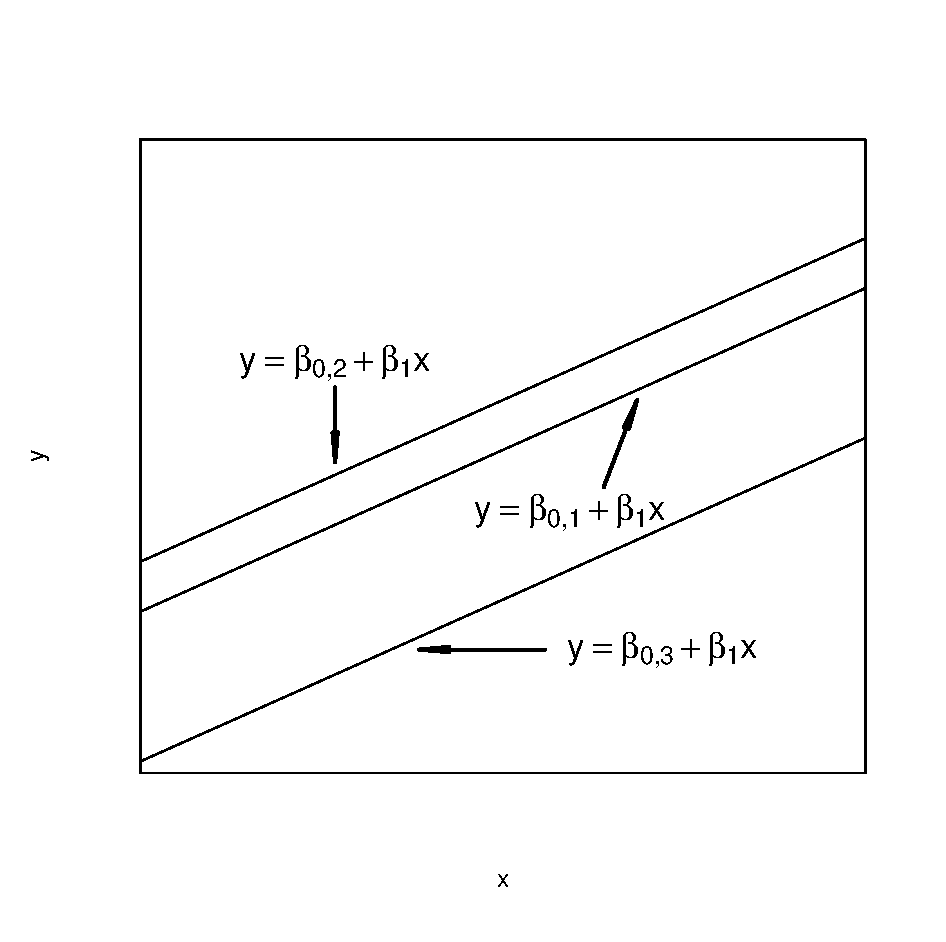
\includegraphics[width=1\textwidth,angle=0,scale=0.45]{Chapter4/Fig4_5A.ps}
    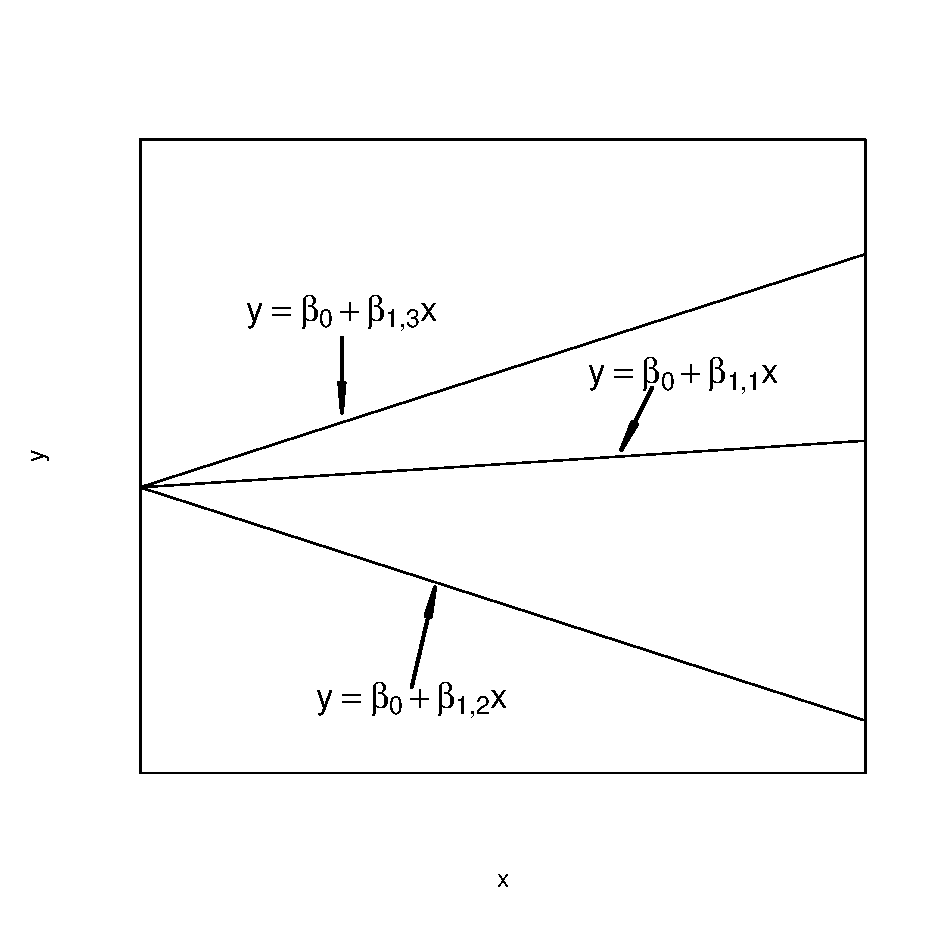
\includegraphics[width=1\textwidth,angle=0,scale=0.45]{Chapter4/Fig4_6A.ps} \hfill
     \parbox[t]{2.5in}{\caption{\label{F4:TheoryVarIntConSlope} \small  Plot of the expected response versus the covariate for the regression model
with variable intercept and constant slope.}} \hfill
    \parbox[t]{2.5in}{\caption{\label{F4:TheoryConIntVarSlope} \small  Plot of the expected response versus the covariate for the regression model
with constant intercept and variable slope.}}
  \end{center}
\end{figure}


\begin{figure}[htp]
  \begin{center}
    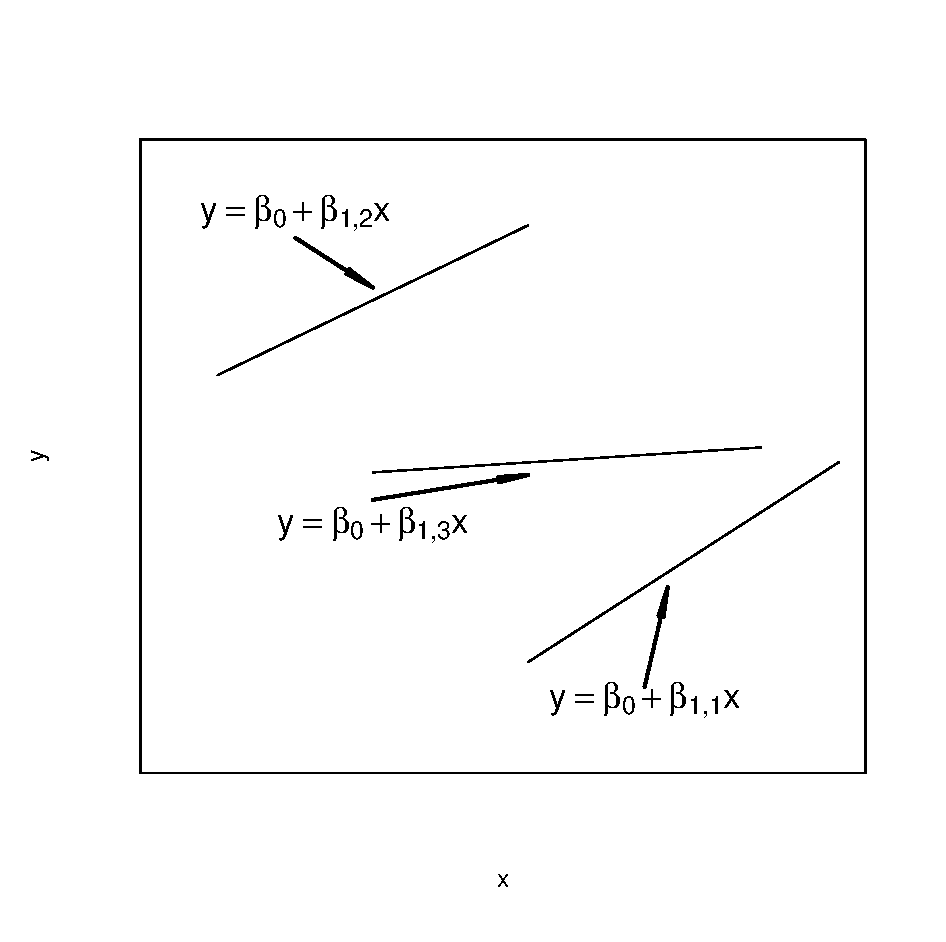
\includegraphics[width=1\textwidth,angle=0,scale=0.5]{Chapter4/Fig4_7A.ps}
    \caption{\label{F4:TheoryVarIntVarSlope} \small  Plot of the expected response versus the covariate for the regression model
with variable intercept and variable slope.}
  \end{center}
\end{figure}

For each model presented in Table \ref{T4:OneFactorCovariate},
parameter estimates can be calculated using the method of least
squares. As usual, this means writing the expected response, E
$y_{ij}$, as a function of known variables and unknown parameters.
Then, for candidate estimates of the parameters, an error sum of
squares can be calculated and minimized over all candidate
estimates. For the regression model with variable intercept and
constant slope, the least squares estimates can be expressed
compactly as:

\begin{equation*}
b_1=\frac{\sum_{j=1}^{c}\sum_{i=1}^{n_{j}}(x_{ij}-\bar{x}_{j})(y_{ij}-\bar{%
y}_{j})}{\sum_{j=1}^{c}\sum_{i=1}^{n_{j}}(x_{ij}-\bar{x}_{j})^{2}}
\end{equation*}

\noindent and $b_{0,j}=\bar{y}_{j}-b_1\bar{x}_{j}$. Similarly, the
least squares estimates for the regression model with variable
intercept and slope can be expressed as:

\begin{equation*}
b_{1,j}=\frac{\sum_{i=1}^{n_{j}}(x_{ij}-\bar{x}_{j})(y_{ij}-\bar{y}_{j})}{%
\sum_{i=1}^{n_{j}}(x_{ij}-\bar{x}_{j})^{2}}
\end{equation*}

\noindent and $b_{0,j}=\bar{y}_{j}-b_1\bar{x}_{j}$. With these
parameter estimates, fitted values may be calculated.

For each model, the error sum of squares is defined as the sum of
squared deviations between the observation and the corresponding
fitted values, that is,

\begin{equation*}
\text{Error
SS}=\sum_{j=1}^{c}\sum_{i=1}^{n_{j}}(y_{ij}-\hat{y}_{ij})^{2}.
\end{equation*}

\noindent Fitted values are defined to be the expected response with
the unknown parameters replaced by their least squares estimates.
For example, for the regression model with variable intercept and
constant slope the fitted values are
$\hat{y}_{ij}=b_{0,j}+b_1x_{ij}$.

\linejed

\textbf{Example. Hospital Charges - Continued.} To illustrate, we
now consider the Hospital Charges case study introduced in Section
4.3. To streamline the presentation, we now consider only costs
associated with three diagnostic related groups (DRGs), DRG \#209,
DRG \#391 and DRG \#430.

The covariate, $x$, is the natural logarithm of the number of
discharges. In ideal settings, hospitals with more patients enjoy
lower costs due to economies of scale. In non-ideal settings,
hospitals may not have excess capacity and thus, hospitals with more
patients have higher costs. One purpose of this analysis is to
investigate the relationship between hospital costs and hospital
utilization.

Recall that our measure of hospital charges is the logarithm of
costs per discharge $(y)$. The scatter plot in Figure
\ref{F4:CostperNumber} gives a preliminary idea of the relationship
between $y$ and $x$. We note that there appears to be a negative
relationship between $y$ and $x$.

The negative relationship between $y$ and $x$ suggested by Figure
\ref{F4:CostperNumber} is misleading and is induced by an
\textit{omitted variable}, the category of the cost (DRG). To see
the joint effect of the categorical variable DRG and the continuous
variable $x$, in Figure \ref{F4:DRGbyNumber} is a plot of $y$ versus
$x$ where the plotting symbols are codes for the level of the
categorical variable. From this plot, we see that the level of cost
varies by level of the factor DRG. Moreover, for each level of DRG,
the slope between $y$ and $x$ is either zero or positive. The slopes
are not negative, as suggested by Figure \ref{F4:CostperNumber}.

\begin{figure}[htp]
  \begin{center}
    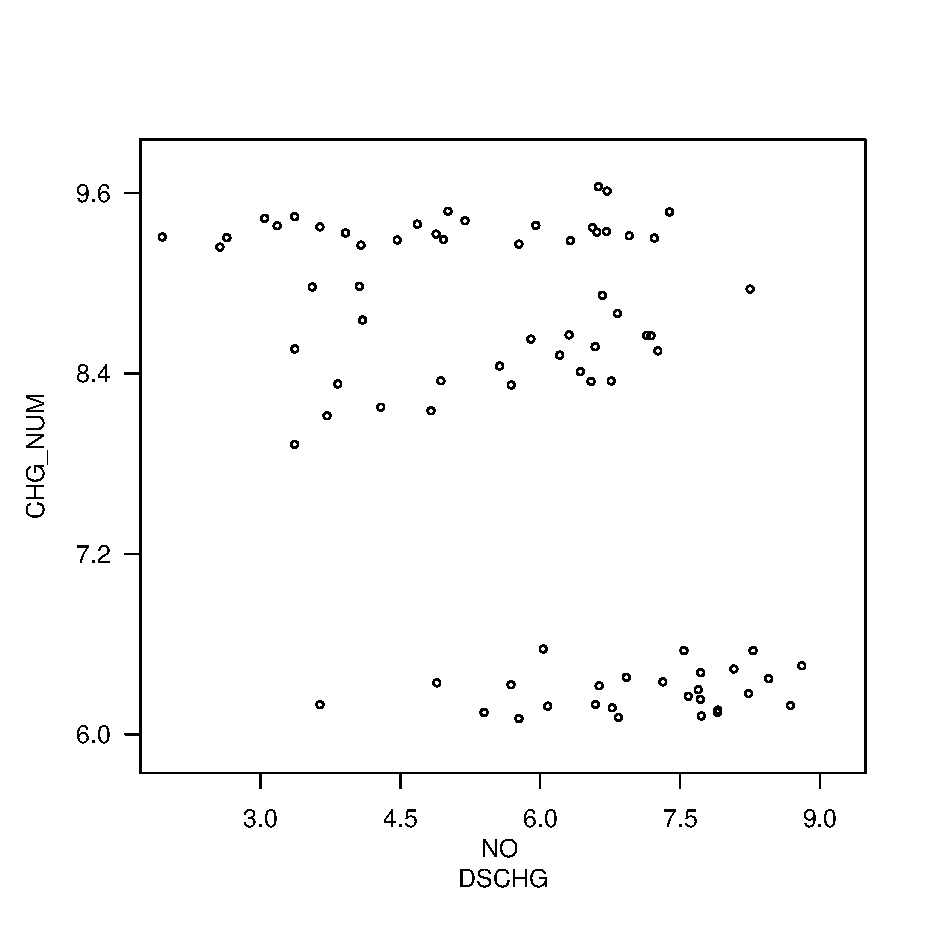
\includegraphics[width=1\textwidth,angle=0,scale=0.45]{Chapter4/Fig4_8A.ps}
    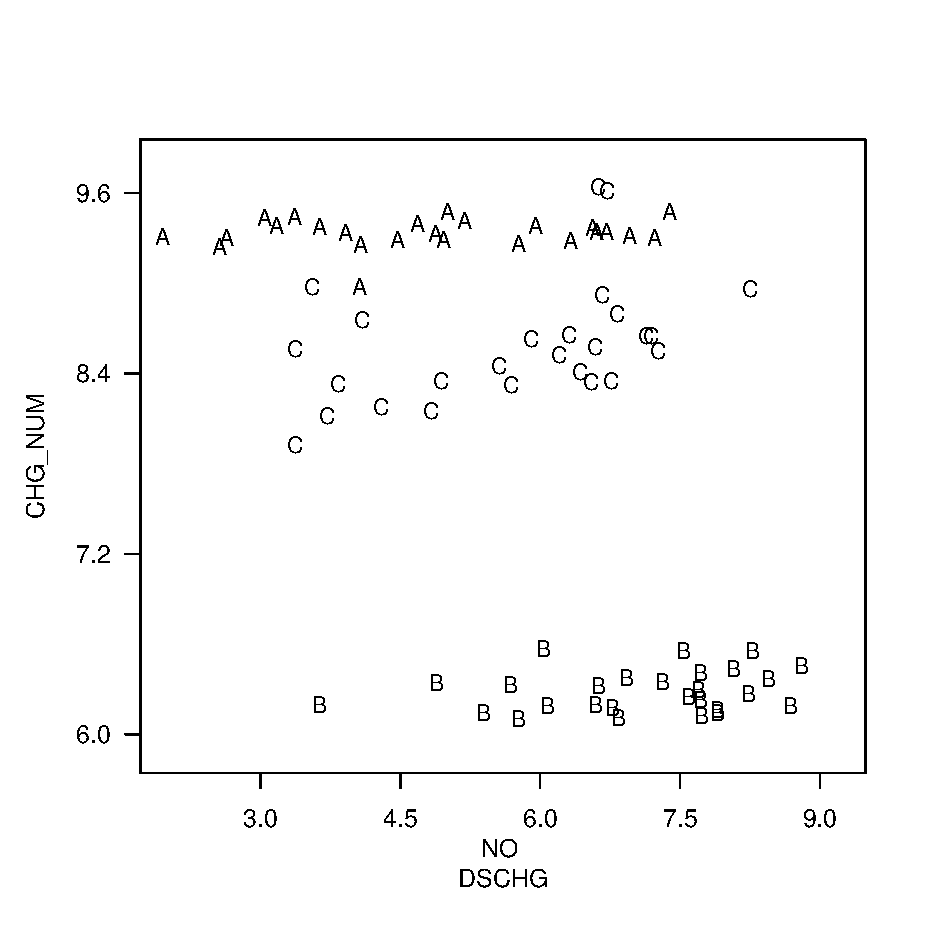
\includegraphics[width=1\textwidth,angle=0,scale=0.45]{Chapter4/Fig4_9A.ps} \hfill
    \parbox[t]{2.5in}{\caption{\label{F4:CostperNumber} \small  Plot of natural logarithm of cost per discharge versus natural
logarithm of the number of discharges.}} \hfill
    \parbox[t]{2.5in}{\caption{\label{F4:DRGbyNumber} \small  Letter plot of natural logarithm of cost per discharge versus natural
logarithm of the number of discharges by DRG. Here, A is for DRG
\#209, B is for DRG \#391 and C is for DRG \#430.}}
  \end{center}
\end{figure}


\scalefont{0.7}  \begin{center}  \begin{table}[h]
\caption{\label{T4:DRGModels} Degree of Freedom and Error Sum of
Squares of Several Models to Represent One Factor and One Covariate
for the DRG Example}
\begin{tabular}{lccrcc}
\hline & Model & Error & Error  &  & Error  \\
& degrees & degrees
& Sum & $R^2$  & Mean \\
Model Description & of freedom & of freedom & of Squares & (\%) &
Square
\\ \hline
One factor ANOVA & 2 &
76 & \multicolumn{1}{r}{$9.396$} & \multicolumn{1}{r}{$%
93.3$} & \multicolumn{1}{r}{$0.124$} \\
Regression with constant intercept & 1 & 77 &
\multicolumn{1}{r}{$115.059$} &
\multicolumn{1}{r}{$18.2$} & \multicolumn{1}{r}{$1.222$} \\
~~~and slope & & & & &  \\
Regression with variable intercept &3 & 75 &
\multicolumn{1}{r}{$7.482$} &
\multicolumn{1}{r}{$94.7$} & \multicolumn{1}{r}{$0.100$} \\
~~~and constant slope &  & &  &  &  \\
Regression with constant intercept & 3 & 75 &
\multicolumn{1}{r}{$14.048$} &
\multicolumn{1}{r}{$90.0$} & \multicolumn{1}{r}{$0.187$} \\
~~~and variable slope &  &  &  &  & \\
Regression with variable intercept & 5 & 73 &
\multicolumn{1}{r}{$5.458$} &
\multicolumn{1}{r}{$96.1$} & \multicolumn{1}{r}{$0.075$} \\
~~~and slope &  & & &  &  \\
\hline
\end{tabular}

\end{table}  \end{center} \scalefont{1.4286}


Each of the five models defined in Table \ref{T4:OneFactorCovariate}
was fit to this subset of the Hospital case study. The summary
statistics are in Table \ref{T4:DRGModels}. For this data set, there
are $n=79$ observations and $c=3$ levels of the DRG factor. For each
model, the model degrees of freedom is the number of model
parameters minus one. The error degrees of freedom is the number of
observations minus the number of model parameters.


Using binary variables, each of the models in Table
\ref{T4:OneFactorCovariate} can be written in a regression format.
As we have seen in Section 4.2, when a model can be written as a
subset of another, larger model, we have formal testing procedures
available to decide which model is more appropriate. To illustrate
this testing procedure with our DRG example, from Table
\ref{T4:DRGModels} and the associated plots, it seems clear that the
DRG factor is important. Further, a $t$-test, not presented here,
shows that the
covariate $x$ is important. Thus, let's compare the full model E $%
y_{ij}=\beta_{0,j}+\beta_{1,j}x$ to the reduced model E
$y_{ij}=\beta_{0,j}+\beta_1x$. In other words, is there a different
slope for each DRG?

Using the notation from Section 4.2, we call the variable intercept
and slope the full model. Under the null hypothesis, $H_0:
\beta_{1,1}=\beta_{1,2}=\beta_{1,3}$, we get the variable intercept,
constant slope model. Thus, using the $F$-ratio in equation
(\ref{E4:FratioErrSumSquares}), we have

\begin{equation*}
F\text{-ratio}=\frac{(Error~SS)_{reduced}-(Error~SS)_{full}}{ps_{full}^{2}}=\frac{{7.482-5.458}}{2(0.075)}=13.535.
\end{equation*}

\noindent The 95th percentile from the $F$-distribution with
$df_1=p=2$ and $df_2=(df)_{full}=73$ is approximately 3.13. Thus,
this test leads us to reject the null hypothesis and declare the
alternative, the regression model with variable intercept and
variable slope, to be valid.

\linejed

\subsubsection*{General Linear Model}

In Section 4.1, we saw that we only use $c-1$ indicator variables to
represent a categorical variable with $c$ levels. Similarly, in
Section 4.3 we saw that the one factor ANOVA model could be
expressed as a regression model with $c$ indicator variables.
However, if we had attempted to estimate the model in equation
(\ref{E4:OneFactorTau}), the method of least squares would not have
arrived at a unique set of regression coefficient estimates. The
reason is that, in equation (\ref{E4:OneFactorTau}), each
explanatory variable can be expressed as a
linear combination of the others. For example, observe that $%
x_{c}=1-(x_1+x_2+\ldots \ +x_{c-1})$.

The fact that parameter estimates are not unique is a drawback, but
not an
overwhelming one. In fact, we now introduce the \textit{general linear model}%
,

\begin{equation} \label{E4:GeneralLinearModel}
y=\beta_0+\beta_1x_1+\ldots \ +\beta_kx_k + \varepsilon,
\end{equation}

\noindent where $\{\varepsilon_i\}$ is a random sample from an
unknown population with mean zero. We follow standard terminology
and view the linear regression model as a special case of the
general linear model. To distinguish the two sets of models, we
assume that the explanatory variables are not linear combinations of
one another in the linear regression model context. This restriction
is not made in the general linear model case. To illustrate, the
models in equations (\ref{E4:OneFactorTau}) and (4.13) are examples
of general linear models that are not regression models.

In the linear regression model case, the assumption that the
explanatory variables are not linear combinations of one another
means that we can compute unique estimates of the regression
coefficients using the method of least squares. In the general
linear model case, the parameter estimates need not be unique.
However, an important feature of the general linear model is that
the resulting fitted values turn out to be unique, using the method
of least squares.

Specifically, suppose that we are considering the model in equation
(4.15) and, using the method of least squares, our regression
coefficient estimates are $b_0^{o},b_1^{o},\ldots ,b_k^{o}$. This
set of regression coefficients estimates minimizes our error sum of
squares, but there are other sets of coefficients that also minimize
the error sum of squares. The fitted values are computed as
$\hat{y}_i=b_0^{o}+b_1^{o}x_{i1}+\ldots \ +b_k^{o}x_{ik}$. It can be
shown that the resulting fitted values are unique, in the sense that
any set of coefficients that minimize the error sum of squares
produce the same fitted values.

Thus, for a set of data and a specified general linear model, fitted
values are unique. Because residuals are computed as observed
responses minus fitted values, we have that the residuals are
unique. Because residuals are unique, we have the error sums of
squares are unique. Thus, it seems reasonable, and is true, that we
can use the general test of hypotheses described in Section 4.2 to
decide whether collections of explanatory variables are important.

To summarize, for general linear models, parameter estimates are not
unique and thus not meaningful. An important part of regression
models is the interpretation of regression coefficients. This
interpretation is not necessarily available in the general linear
model context. However, for general linear models, we may still
discuss the important of an individual variable or collection of
variables through partial \textit{F}-tests. Further, fitted values,
and the corresponding exercise of prediction, works in the general
linear model context. The advantage of the general linear model
context is that we need not worry about the type of restrictions to
impose on the parameters. Although not the subject of this text,
this advantage is particularly important in complicated experimental
designs used in the life sciences. Searle (1987) is one reference
for these designs and for further details of the general linear
model. The reader will find that general linear model estimation
routines are widely available in statistical software packages
available on the market today.


\section{Two Factor ANOVA Model}

Suppose that we now wish to consider two categorical explanatory
variables, or factors. We first establish some notation in the
context of the following example.

\linejed

\textbf{Example: Machine Run Times.} In this example, the response
of interest is the length of time it takes a machine to complete a
certain benchmark test. The explanatory variables considered are the
type of machine and the type of person operating the machine. For
convenience, think of the operator as either experienced or
inexperienced (a rookie). We refer to the operator as Factor 1 and
the type of machine as Factor 2, although these designations are
interchangeable. Table \ref{T4:MachineTimes} presents the sample
data.

\scalefont{0.9}  \begin{center}  \begin{table}[h]
\caption{\label{T4:MachineTimes} Hypothetical Run Times of Three
Machines by Two Operators}
\begin{tabular}{cccc}
\hline & \multicolumn{2}{c}{Operator (Factor 1)} &  \\ \cline{2-3}
Machine (Factor 2) & Rookie & Experienced & Machine Averages \\
\hline 1 & \multicolumn{1}{r}{$14,12$} & \multicolumn{1}{r}{$10,12$}
&
\multicolumn{1}{l}{$\ \ \ \ \bar{y}_{\cdot 1\cdot }=12$} \\
2 & \multicolumn{1}{r}{$15,16$} & \multicolumn{1}{r}{$9,12$} &
\multicolumn{1}{l}{$\ \ \ \ \bar{y}_{\cdot 2\cdot }=13$} \\
3 & \multicolumn{1}{r}{$8,10$} & \multicolumn{1}{r}{$7,7$} &
\multicolumn{1}{l}{$\ \ \ \ \bar{y}_{\cdot 3\cdot }=8$} \\ \hline
Operator Average & $\bar{y}_{1..}=12.5$ & $\bar{y}_{2..}=9.5$ & $\bar{y}%
_{3..}=11$ \\ \hline
\end{tabular}

\end{table}  \end{center}  \scalefont{1.1111}


Extending the notation introduced in Section 4.3, we use $y_{ijk}$
to denote the $k$th observation of the $i$th operator of the $j$th
machine. We suppose that there are $K=2$ observations for each
combination of the $I=2$ types of operators and $c=3$ types of
machines. Thus, there are $n=IcK=2(3)2=12$ observations in total.

As in Section 4.3, an important issue that can be addressed with
this data is whether the (population) mean run times differ among
machine types. To this end, we define the average for each machine,
$j=1,2,3,$ using $ \bar{y}_{\cdot j\cdot
}=\frac{1}{IK}\sum_{i=1}^{I}\sum_{k=1}^{K}y_{ijk}\text{ }.$ Here,
the notation $\{\cdot j\cdot \}$ in the subscript means sum over $%
i=1,\ldots ,I$, leave $j$ fixed, and sum over $k=1,\ldots ,K$. One
goal of this section is to explain part of the unknown variability
in terms of the type of operator. To this end, we can define the
average for each operator, $i=1,2$, using $\bar{y}_{i\cdot \cdot
}=\frac{1}{cK}\sum_{j=1}^{c}\sum_{k=1}^{K}y_{ijk}\text{ }.$
 It is also convenient for subsequent analyses to define
the average over each combination of operator and machine
$\bar{y}_{ij\cdot }=\frac{1}{K}\sum_{k=1}^{K}y_{ijk}. $

Table \ref{T4:MachineTimes} shows that there may be a difference
between the two types of operators as well as the three types of
machines. Are the differences in sample mean run times due to
sampling variability or are they due to differences in population
mean run times? How does accounting for the type of operator help
understand the performance of different machine types? To respond to
these and related questions, we now introduce two models of
variability.

\linejed

\subsubsection*{Model Assumptions and Analysis - Additive Model}

If we wish to put two categorical, or attribute, variables together
in one model, there are two basic approaches. These are called
\textit{additive} and \textit{interaction} models, respectively. To
illustrate these two approaches, we begin with the simpler additive
model.

Using the one factor formulation in equation
(\ref{E4:OneFactorTau}), we interpret the parameter $\mu $ to be the
population mean and $\tau_{j}$ to be the difference due to the $j$th
level of Factor 2. Similarly, we introduce the parameter $\beta_i$
to be interpreted as the difference due to the $i$th level of Factor
1. With these parameters, the two factor additive model is

\begin{equation}  \label{E4:TwoFactorTau}
y_{ijk}=\mu +\beta_i+\tau_{j}+\varepsilon_{ijk}
\end{equation}%
where $i=1,\ldots ,I,j=1,\ldots ,c,$ and $k=1,\ldots ,K$. The
errors, $ \{\varepsilon_{ijk}\}$, are assumed to be random,
independent draws from a common population with mean zero and
variance $\sigma ^{2}$.

As with the one factor model, we again need to impose certain
restrictions on the factor differences. So that all levels of each
factor are treated in the same fashion, we require

\begin{equation}\label{E4:Restrictions}
\beta_1 + \beta_2 + \ldots + \beta_I = 0 ~ ~\mathrm{and}~ ~\tau_1 +
\tau_2 + \ldots + \tau_c = 0.
\end{equation}

Note that in this section we do not use the number of observations
in our restrictions as we did in Section 4.3. This is because of the
fact that in this section the data are assumed to be
\textit{balanced}. That is, for each combination of levels of
Factors 1 and 2, we assume that there are an equal number,
\textit{K}, of observations available. This assumption is made
primarily in order to simplify the presentation. It is possible to
present the formulas where the number of observations may vary by
combinations of levels (see, for example, Searle, 1987). Instead, in
this chapter, we handle unbalanced data a special case of the
general linear model, introduced in Section 4.5.

The least squares parameter estimates are determined by minimizing
the sum of squares

\begin{equation*}
SS(\hat{\mu},\hat{\beta}_1,\ldots ,\hat{\beta}_{I},
\hat{\tau}_1,\ldots
,\hat{\tau}_{c})=\sum_{i=1}^{I}\sum_{j=1}^{c}\sum_{k=1}^{K}(y_{ijk}-(\hat{\mu}+
\hat{\beta}_i+\hat{\tau}_{j}))^{2}.
\end{equation*}

\noindent Here, $\hat{\mu},\hat{\beta}_1,\ldots
,\hat{\beta}_{I},\hat{\tau}_1,\ldots ,\hat{\tau}_{c}$ are candidate
estimates of $\mu ,\beta_1,\ldots ,\beta_I,\tau _1,\ldots ,\tau_c$.
Minimizing this sum of squares subject to the restrictions in
equation (\ref{E4:Restrictions}), the least squares estimates are

\begin{equation}  \label{E4:TwoFactorEstimates}
\hat{\mu}=\bar{y}_{\cdot \cdot \cdot },\text{ \ \ }\hat{\beta}_i=\bar{y}%
_{i\cdot \cdot }-\bar{y}_{\cdot \cdot \cdot },\text{ \ and }\hat{\tau}_{j}=%
\bar{y}_{\cdot j\cdot }-\bar{y}_{\cdot \cdot \cdot }\text{ .}
\end{equation}

Thus, the variability still unaccounted for, after the introduction
of the
parameters $\mu $, $\beta $ and $\tau $, is summarized by%
\begin{eqnarray}\label{E4:TwoFactorErrorSS}
\text{Error SS} &=&SS(\hat{\mu},\hat{\beta}_1,\ldots ,\hat{\beta}_{I},\hat{%
\tau}_1,\ldots ,\hat{\tau}_{c})=\sum_{i=1}^{I}\sum_{j=1}^{c}%
\sum_{k=1}^{K}(y_{ijk}-(\hat{\mu}+\hat{\beta}_i+\hat{\tau}_{j}))^{2}.
\notag \\
&=&\sum_{i=1}^{I}\sum_{j=1}^{c}\sum_{k=1}^{K}(y_{ijk}-\bar{y}_{i\cdot
\cdot }-\bar{y}_{\cdot j\cdot }+\bar{y}_{\cdot \cdot \cdot })^{2}
\end{eqnarray}

To account for each source of the variability, consider the
decomposition

\begin{equation}  \label{E9:TwoFactorDecomp}
y_{ijk}-\bar{y}_{\cdot \cdot \cdot }=(\bar{y}_{\cdot i\cdot
}-\bar{y}_{\cdot \cdot \cdot })+(\bar{y}_{\cdot j\cdot
}-\bar{y}_{\cdot \cdot \cdot })+(y_{ijk}-\bar{y}_{i\cdot \cdot
}-\bar{y}_{\cdot j\cdot }+\bar{y}_{\cdot \cdot \cdot }).
\end{equation}

\begin{center}
(1) \ \ \ \ \ \ \ \ \ \ \ \ \ \ (2)\qquad\ \ \ \ \ \ \ \ (3) \ \ \ \
\ \ \ \ \ \ \ \ \ \ \ \ \ \ \ \ \ \ \ (4) \ \ \ \ \ \ \ \ \
\end{center}

Interpret this equation as (1) the total deviation equals (2) the
deviation explained by Factor 1 plus (3) the deviation explained by
Factor 2 plus (4) the unexplained deviation. Squaring each side of
equation (\ref{E9:TwoFactorDecomp}) and summing over all
observations yields

\begin{equation*}
\text{Total SS = Factor 1 SS + Factor 2 SS + Error SS}.
\end{equation*}

\noindent Here, Error SS is defined in equation
(\ref{E4:TwoFactorErrorSS}) and, with equation
(\ref{E4:TwoFactorEstimates}),

\begin{subequations}
\begin{eqnarray}
\text{Total SS} &=&\sum_{i=1}^{I}\sum_{j=1}^{c}\sum_{k=1}^{K}(y_{ijk}-\bar{y}%
_{\cdot \cdot \cdot })^{2},   \label{E4:TwoFactorTotalSS}\\
\text{Factor 1 SS } &=&cK\sum_{i=1}^{I}(\bar{y}_{j\cdot \cdot }-\bar{y}%
_{\cdot \cdot \cdot })^{2}=cK\sum_{i=1}^{I}\hat{\beta}_i^{2}  \notag \\
\text{Factor 2 SS} &=&IK\sum_{j=1}^{c}(\bar{y}_{\cdot j\cdot }-\bar{y}%
_{\cdot \cdot \cdot })^{2}=IK\sum_{j=1}^{c}\hat{\tau}_{j}^{2}.
\notag
\end{eqnarray}
\end{subequations}

\noindent The variability decomposition is summarized in the
following analysis of variance (ANOVA) table.

\begin{center}
ANOVA Table for Two Factor Additive Model
\begin{tabular}{lccc}
\hline Source & Sum of Squares & $\mathit{df}$ & Mean Square \\
\hline
Factor 1 & Factor 1 SS & $I-1$ & Factor 1 MS \\
Factor 2 & Factor 2 SS & $c-1$ & Factor 2 MS \\
Error & Error SS & $n-(I+c-1)$ & Error MS \\
Total & Total SS & $n-1$ &  \\ \hline
\end{tabular}
\end{center}

Again, the mean squares (MS) column is defined by the sum of squares
(SS) column divided by the degrees of freedom (\textit{df}) column.
Thus, Factor 1 MS $\equiv $ (Factor 1 SS)/$(I-1)$, Factor 2 MS
$\equiv $ (Factor 2 SS)/$(c-1)$ and Error MS $\equiv $ (Error
SS)/$(n-(I+c-1))$. To understand the degrees of freedom column for
the errors, first note that there are $1+I+c$ parameters, one for
$\mu $, $I$ for $\beta $ and $c$ for $\tau $. However, there are two
restrictions on $\{\beta_i\}$ and $\{\tau_{j}\}$, resulting in
$I+c-1$ free parameters. Thus, the error degrees of freedom follows
the same rule as all regression models, the number of observations,
$n$, minus the number of (free) parameters, $I+c-1$.

To illustrate, Table \ref{T4:ANOVATwoFactor} presents results for
the data in Table \ref{T4:MachineTimes}.

\scalefont{0.9}  \begin{center}  \begin{table}[h]
\caption{\label{T4:ANOVATwoFactor} ANOVA Table for Two Factor
Additive Model of Hypothetical Run Times}

\begin{tabular}{lccc}
\hline Source & Sum of Squares & \textit{df} & Mean Square \\
\hline Operator (Factor 1) & 27  & 1  & 27 \\
Machine (Factor 2)         & 56  & 2  & 28 \\
Error                      & 17  & 8  & 2.12 \\
Total                      & 100 & 11 &  \\ \hline
\end{tabular}

\end{table}  \end{center}  \scalefont{1.1111}

As before, tests of hypotheses allows us to test formally for
differences among levels of each factor. For example, the notation
H$_0$: $\beta_1=\ldots =\beta_I=0$ stands for the null hypothesis:
all Factor 1 level mean differences are equal to zero. In other
words, this is the hypothesis that there is no difference among
levels of Factor 1. The alternative hypothesis is that at least some
of the means differ from one another. For this test, we examine the
\textit{F}-ratio=(Factor 1 MS)/(Error MS). The null hypothesis is
rejected in favor of the alternative if $F-ratio>F-value. $ Here,
the $F$-value is a percentile from the $F$-distribution with
$df_1=I-1$ and $df_2=n-(I+c-1)$ degrees of freedom. The percentile
is one - significance level. In our machine example, with $df_1=1$
and $df_2=8$, at the 5\% significance level, we have
\textit{F}-value=5.318 from a table of the $F$-distribution. From
Table \ref{T4:ANOVATwoFactor}, we have $\mathit{F}$-ratio
$=27/2.12=12.74$. Because $12.74=F$-ratio $>F$-value $=5.318$, we
reject the null hypothesis and conclude that there is a real
difference between types of operators. This result reinforces our
examination of the data in Table \ref{T4:MachineTimes}.

The test of hypothesis for differences among levels of Factor 2 is
similar. To summarize, consider the Table \ref{T4:TwoFactorTests}.


\scalefont{0.8}  \begin{center}  \begin{table}[h]
\caption{\label{T4:TwoFactorTests} Test of Hypothesis of Differences
Among Levels for Two Factor Additive Model}

\begin{tabular}{ccccc}
\hline & Null & Alternative & Test statistic & Degree of Freedom to
use \\
Factor & hypothesis & hypothesis & ($F$-ratio) & with the $F$-value \\
\hline 1 & H$_0$: $\beta_1=\ldots$ & ~~~H$_a$: At least one  & (Factor 1 MS)/ & $df_1=I-1,$  \\
&  $~~~~=\beta_I=0$ & $
~~~~\beta \neq 0$ & (Error MS) &  $df_2=n-(I+c-1)$\\
2 & H$_0$: $\tau_1=\ldots $  & ~~~H$_a$: At least one  & (Factor 2 MS)/ & $df_1=c-1,$  \\
& $~~~~=\tau_c=0$ &  ~~~~$\tau \neq 0$& (Error MS) &
$df_2=n-(I+c-1)$ \\ \hline
\end{tabular}

\end{table}  \end{center}  \scalefont{1.25}

For example, to test differences among types of machines, we hypothesize H$%
_0$: $\tau_1=\tau_2=\tau_3=0$. To perform the test, we first
calculate \textit{F}-ratio $=$ (Factor 2 MS)/(Error MS) = 28/2.12 =
13.21. From the \textit{F}-table with $df_1=2$ and $df_2=8$, at the
5\% significance level, we have \textit{F}-value = 4.459. Because
$13.21>4.459$, we reject the null hypothesis that there is no
difference among machines.


\subsubsection*{Model Assumptions and Analysis - Interaction Model}

For the two factor additive model, we assumed that we could simply
add together the impact of each variable, together with a population
mean, to form the expected response. However, it may be that reality
is better represented by examining more complicated interactions
between the two factors. For example, in our hypothetical machine
example, it may be that experienced operators run certain types of
machines much faster than inexperienced operators even though, for
other types of machines, experienced operators post only marginally
faster run times.

To accommodate potential interactions, we use the model

\begin{equation}\label{E$:TwoFactorInteraction}
y_{ijk}=\mu_{ij}+\varepsilon_{ijk}.
\end{equation}

\noindent Here, $\mu_{ij}$ represents the mean response for the
$i$th level of Factor 1 and the $j$th level of Factor 2. As with
equation (\ref{E4:OneFactor}), we would like to rewrite this model
into interpretable components. To this end, define

\begin{equation*}
\text{(a) }\mu =\frac{1}{Ic}\sum_{i=1}^{I}\sum_{j=1}^{c}\mu
_{ij}\text{, \ \ (b) }\beta_i=(\frac{1}{c}\sum_{j=1}^{c}\mu
_{ij})-\mu \text{,}
\end{equation*}

\begin{equation*}
\text{(c) }\tau_{j}=(\frac{1}{I}\sum_{i=1}^{I}\mu_{ij})-\mu \text{,\
\ \ (d) }(\beta \tau )_{ij}=\mu_{ij}-\beta_i-\tau_{j}-\mu .
\end{equation*}

\noindent As with the additive model, $\mu $ represents the overall
mean, $\beta_i$ represents Factor 1 differences and $\tau_{j}$
represents Factor 2 differences. We use the term $(\beta \tau
)_{ij}$ to represent the interaction between the two factors.

By substituting the expression for $(\beta \tau )_{ij}$ into
(\ref{E$:TwoFactorInteraction}), we get

\begin{equation} \label{E4:TwoFactorInteractionComponents}
y_{ijk}=\mu +\beta_i+\tau_{j}+(\beta \tau )_{ij}+\varepsilon_{ijk}.
\end{equation}%
\qquad

When comparing equations (\ref{E$:TwoFactorInteraction}) and
(\ref{E4:TwoFactorInteractionComponents}), we see that there are
$Ic$ linear parameters in equation (\ref{E$:TwoFactorInteraction})
even though there are $1+I+c+Ic$ parameters in equation
(\ref{E4:TwoFactorInteractionComponents}). As before, certain
restrictions need to be imposed on the parameters in equation
(\ref{E4:TwoFactorInteractionComponents}) so that these models are
equivalent. The restrictions adopted here are:

\begin{equation*}
\sum_{i=1}^{I}\beta_i=0,\text{ }\sum_{j=1}^{c}\tau_{j}=0,\text{ }%
\sum_{i=1}^{I}(\beta \tau )_{ij}=0\,,\text{ \ for each }j,
\end{equation*}

\begin{equation*}
\text{and }\sum_{j=1}^{c}(\beta \tau )_{ij}=0,\text{ \ for each }i.
\end{equation*}

\noindent These restrictions impose $I+c+1$ constraints, so that
there are $Ic$ free parameters in each expression.

Parameter estimation and partitioning the variability of the
interaction model parallel the development of the additive model.
Thus, only a brief outline is presented here. The least squares
estimates of $\mu $, $\beta_i $ and $\tau_{j}$ are the same as
presented in equation (\ref{E4:TwoFactorEstimates}). The least
squares estimate of $(\beta \tau )_{ij}$ turns out to be $\bar{y}_{ij\cdot }-%
\bar{y}_{i\cdot \cdot }-\bar{y}_{\cdot j\cdot }+\bar{y}_{\cdot \cdot \cdot }$%
. Partitioning the variability yields:

\begin{center}
Total SS = Factor 1 SS + Factor 2 SS + Interaction SS + Error SS.
\end{center}

Here, Total SS, Factor 1 SS and Factor 2 SS are defined in equation
(\ref{E4:TwoFactorTotalSS}) and

\begin{equation*}
\text{Interaction SS}=K\sum_{i=1}^{I}\sum_{j=1}^{c}(\bar{y}_{ij\cdot }-\bar{y%
}_{i\cdot \cdot }-\bar{y}_{\cdot j\cdot }+\bar{y}_{\cdot \cdot \cdot
})^{2}
\end{equation*}

\begin{equation*}
\text{and \ \  Error SS}=\sum_{i=1}^{I}\sum_{j=1}^{c}\sum_{k=1}^{K}(y_{ijk}-%
\bar{y}_{ij\cdot })^{2}.
\end{equation*}

These results can be summarized in the following analysis of
variance table.

\scalefont{0.9}
\begin{center}
\begin{tabular}{cccc}
\multicolumn{4}{c}{\textbf{\ }ANOVA Table for Two Factor Interaction Model} \\

\hline Source & Sum of Squares & \textit{df} & Mean Square \\ \hline
\multicolumn{1}{l}{Factor 1} & \multicolumn{1}{l}{Factor 1 SS} &
$I-1$ &
\multicolumn{1}{l}{Factor 1 MS} \\
\multicolumn{1}{l}{Factor 2} & \multicolumn{1}{l}{Factor 2 SS} &
$c-1$ &
\multicolumn{1}{l}{Factor 2 MS} \\
\multicolumn{1}{l}{Interaction} & \multicolumn{1}{l}{Interaction SS} & $%
(I-1)(c-1)$ & \multicolumn{1}{l}{Interaction MS} \\
\multicolumn{1}{l}{Error} & \multicolumn{1}{l}{Error SS} & $n-Ic$ &
\multicolumn{1}{l}{Error MS} \\
\multicolumn{1}{l}{Total} & \multicolumn{1}{l}{Total SS} & $n-1$ &
\multicolumn{1}{l}{} \\ \hline
\end{tabular}
\end{center}
\scalefont{1.1111}

\noindent We remark that the degrees of freedom for the unexplained
variability, the Error Sum of Squares, is the number of
observations, \textit{n}, minus the number of free parameters,
\textit{Ic}.

From the error degrees of freedom, we see that it is necessary to
have more than one observation for each combination of the two
factors. That is, \textit{K} must be greater than one. If \textit{K}
equals one, then the number of observations, $n=IcK$, equals the
number of parameters. In this case, the data fits the model
perfectly, there is no error, and there are no degrees of freedom
available for the error sum of squares. This is not the case in the
additive model where we may have $K=1$. This is because the error
degrees of freedom, $n-(I+c+1)=IcK-(I+c+1)$, can be greater than
zero even if $K=1$.

To test whether or not the interaction terms are important, we hypothesize H$%
_0$: all $(\beta \tau )_{ij}$'s $=0$ versus the alternative hypothesis H$%
_a$: at least one $(\beta \tau )_{ij}\neq 0$. This null hypothesis
is rejected in favor of the alternative if $F$-ratio = (Interaction
MS)/(Error MS) $>$ $F$-value, where the $F$-value is a (1 -
significance level) percentile from the $F$-distribution with
$df_1=(I-1)(c-1)$ and $df_2=n-Ic$ degrees of freedom. To illustrate
this test, consider the machine run data presented in Table
\ref{T4:MachineTimes}. Table \ref{T4:TwoFactorANOVARunTimes}
presents the analysis of variance for the two factor interaction
model fit of this example.

\scalefont{0.9}  \begin{center}  \begin{table}[h]
\caption{\label{T4:TwoFactorANOVARunTimes} ANOVA Table for Two
Factor Interaction Model of Hypothetical Run Times}
\begin{tabular}{lccc}
\hline Source & Sum of Squares & \textit{df} & Mean Square \\ \hline
Operator (Factor 1)      & 27  & 1  & 27 \\
Machine (Factor 2)       & 56  & 2  & 28 \\
Interaction              & 6   & 2  & 3 \\
Error                    & 11  & 6  & 1.83 \\
Total                    & 100 & 11 &\\ \hline
\end{tabular}
\end{table}  \end{center}  \scalefont{1.1111}

To test for the presence of significant interaction terms, we
compute
$F$-ratio $=3/1.83=1.64$. From an $F$-table with $df_1=2$ and $%
df_2=6$ degrees of freedom, at the 5\% level of significance we have
$F$-value $=5.143$. Thus, we cannot reject the null hypothesis that
the interaction effects are significantly different from zero.

It is also possible to test the hypothesis of no differences among
factor levels using the interaction model. One would simply use the
procedures outlined in Table \ref{T4:TwoFactorTests} for the
additive model but using the interaction model error mean squares
and degrees of freedom. However, the interpretation of this
decision-making procedure is not clear. Under the interaction model,
the terms $(\beta \tau )_{ij}$ represent the interaction, or joint
effect, of the $i$th level of Factor 1 and the $j$th level of Factor
2. With terms of this type present, it is difficult to interpret the
decision that either Factor 1 or Factor 2 is not important.

Deciding whether or not a factor is important may be the main goal
of the data analysis. One way to address this is to test first
whether or not the interaction terms are important. If not, as in
the machine example above, the analyst can then represent the data
using the additive model where the importance of a factor can be
tested. It is important to note that with this procedure, we are
fitting two models to the data and that the usual caveats apply.

\subsubsection*{Link with Regression}

In this subsection, we show how to connect the two factor ANOVA
models to a regression model using binary variables. To this end,
for the \textit{I} levels of Factor 1, define $x_{1,i}$ to be a one
if the observation falls in the $i$th level of Factor one and is
zero otherwise. Similarly, define $x_{2,j}$ to be an indicator of
the $j$th level of Factor 2. With this notation, we can re-express
the two factor additive model in equation (\ref{E4:TwoFactorTau}) as

\begin{equation} \label{E4:TwoFactorRegression}
y=\mu +\sum_{i=1}^{I}\beta_ix_{1,i}+\sum_{j=1}^{c}\tau_{j}x_{2,j} +
\varepsilon.
\end{equation}

For example, for an observation falling in the third level of Factor
1 and the fourth level of Factor 2, we have $x_{1,3}=1$, $x_{2,4}=1$
and all other $x$'s $=0$. Thus, equation
(\ref{E4:TwoFactorRegression}) reduces to $y_{23,k}=\mu +\beta
_3+\tau_{4}+\varepsilon_{34,k}$, as in equation
(\ref{E4:TwoFactorInteractionComponents}).

As with equation (\ref{E4:TwoFactorInteractionComponents}), certain
restriction must be applied to the parameters. In the ANOVA models,
the restriction is that the sum over levels of the parameters is
zero. For regression routines, it is more straightforward to drop an
explanatory indicator variable from each factor. Dropping the last
variable of each factor yields

\begin{equation*}
y\equiv \mu +\sum_{i=1}^{I-1}\beta_ix_{1,i}+\sum_{j=1}^{c-1}\tau
_{j}x_{2,j} + \varepsilon.
\end{equation*}

\noindent Here, we interpret $\mu$ to be the mean response for the
$I$th level of Factor 1 and the $c$th level of Factor 2. The
parameter $\beta_i$ is interpreted to be the difference in mean
responses between the $i$th and the $I$th levels of Factor 1.
Similarly, the parameter $\tau_{j}$ is interpreted to be the
difference in mean responses between the $j$th and the $c$th levels
of Factor 2. Thus, for the model fit, it does not matter which
variables are dropped from the equation. However, it does matter
when interpreting the parameters, and their resulting estimates.

The case of the two factor interaction model is similar. We can
rewrite equation (\ref{E4:TwoFactorRegression}) as

\begin{equation} \label{E4:TwoFactorRegressionInteract}
y=\mu +\sum_{i=1}^{I}\beta_ix1,i+\sum_{j=1}^{c}\tau
_{j}x_{2,j}+\sum_{i=1}^{I}\sum_{j=1}^{c}(\beta \tau
)_{ij}x_{1,i}x_{2,j}+ \varepsilon.
\end{equation}

\noindent Dropping one indicator variable from each factor yields
the analogous regression model

\begin{equation}  \label{E4:TwoFactorRegressionDrop}
y=\mu +\sum_{i=1}^{I-1}\beta_ix_{1,i}+\sum_{j=1}^{c-1}\tau
_{j}x_{2,j}+\sum_{i=1}^{I-1}\sum_{j=1}^{c-1}(\beta \tau
)_{ij}x_{1,i}x_{2,j} + \varepsilon.
\end{equation}

Again, equation (\ref{E4:TwoFactorRegressionInteract}) must be
estimated using restricted parameters. Equation
(\ref{E4:TwoFactorRegressionDrop}) provides an equivalent
formulation without the need to restrict the parameters. To
illustrate equation (\ref{E4:TwoFactorRegressionDrop}), consider our
machine example with $I=2$ and $c=3$. In this case, equation
(\ref{E4:TwoFactorRegressionDrop}) reduces to:

\begin{equation*}
y=\mu +\beta_1x_{1,1}+\tau_1x_{2,1}+\tau_2x_{2,2}+(\beta \tau
)_{11}x_{1,1}x_{2,1}+(\beta \tau )_{12}x_{1,1}x_{2,2}+e.
\end{equation*}

\noindent This is a multiple linear regression model with five
independent variables.



\section{Further Reading and References}


\textbf{Chapter References}

\begin{multicols}{2}

\scalefont{0.9}

Keeler, Emmett B., and  John E. Rolph (1988). The demand for
episodes of treatment in the Health Insurance Experiment.
\emph{Journal of Health Economics} 7: 337-367.


\scalefont{1.1111}

\end{multicols}

\bigskip


\section{Exercises}




\section{Technical Supplement - Matrix Expressions}

\subsection{Expressing Models with Categorical Variables in
Matrix Form}

In Chapter 4, we explored the analysis for models of the form
$\mathbf{y=X}  \boldsymbol \beta + \boldsymbol \varepsilon$ where
$\mathbf{X}$ is a matrix of explanatory variables such that
$\mathbf{X}^{\prime }\mathbf{X}$ is invertible. In this section, we
show how to use this model to form two models with categorical
variables. In the next section, we will consider models where
$\mathbf{X}^{\prime }\mathbf{X}$ need not be invertible.

\textbf{One Categorical Variable Model.} Consider the model with one
categorical variable introduced in Section 4.3, $y_{j}=\mu_{j} +
\varepsilon_{j}.$ In this model, there are $c$ levels of the
categorical variable. As in equation (\ref{E4:OneFactor}), this
model can be written as
\begin{equation*}
y=\mu_1x_1+\mu_2x_2+\ldots +\mu_cx_{c}+\varepsilon.
\end{equation*}
where $x_{j}$ is an indicator variable that the observation falls in the $j$%
th level. Using matrix notation, equation (\ref{E4:OneFactor}) can
be expressed as

\begin{equation}\label{E4:MatrixOneFactor}
\mathbf{y}=%
\begin{bmatrix}
y_{1,1} \\
\cdot  \\
\cdot  \\
\cdot  \\
y_{n_1,1} \\
\cdot  \\
\cdot  \\
\cdot  \\
y_{1,c} \\
\cdot  \\
\cdot  \\
\cdot  \\
y_{n_{c},c}%
\end{bmatrix}%
=%
\begin{bmatrix}
1 & 0 & \cdot \cdot \cdot  & 0 \\
\cdot  & \cdot  & \cdot \cdot \cdot  & \cdot  \\
\cdot  & \cdot  & \cdot \cdot \cdot  & \cdot  \\
\cdot  & \cdot  & \cdot \cdot \cdot  & \cdot  \\
1 & 0 & \cdot \cdot \cdot  & \cdot  \\
\cdot  & \cdot  & \cdot \cdot \cdot  & \cdot  \\
\cdot  & \cdot  & \cdot \cdot \cdot  & \cdot  \\
\cdot  & \cdot  & \cdot \cdot \cdot  & \cdot  \\
0 & 0 & \cdot \cdot \cdot  & 1 \\
\cdot  & \cdot  & \cdot \cdot \cdot  & \cdot  \\
\cdot  & \cdot  & \cdot \cdot \cdot  & \cdot  \\
\cdot  & \cdot  & \cdot \cdot \cdot  & \cdot  \\
0 & 0 & \cdot \cdot \cdot  & 1%
\end{bmatrix}%
\begin{bmatrix}
\mu_1 \\
\cdot  \\
\cdot  \\
\cdot  \\
\mu_c%
\end{bmatrix}%
+%
\begin{bmatrix}
\varepsilon_{1,1} \\
\cdot  \\
\cdot  \\
\cdot  \\
\varepsilon_{n_1,1} \\
\cdot  \\
\cdot  \\
\cdot  \\
\varepsilon_{1,c} \\
\cdot  \\
\cdot  \\
\cdot  \\
\varepsilon_{n_{c},c}%
\end{bmatrix}%
=\mathbf{X\ \boldsymbol \beta + \boldsymbol \varepsilon} \text{\ \ \
\ }
\end{equation}



To make the notation more compact, we write $\mathbf{0}$ and
$\mathbf{1}$ for a column of zeros and ones, respectively. With this
convention, another way to express equation
(\ref{E4:MatrixOneFactor}) is

\begin{center}
\begin{equation}\label{E4:Matrix2OneFactor}
\mathbf{y}=%
\begin{bmatrix}
\mathbf{1}_1 & \mathbf{0}_1 & \cdot \cdot \cdot  & \mathbf{0}%
_1 \\
\mathbf{0}_2 & \mathbf{1}_2 & \cdot \cdot \cdot  & \mathbf{0}%
_2 \\
\cdot  & \cdot  & \cdot \cdot \cdot  & \cdot  \\
\cdot  & \cdot  & \cdot \cdot \cdot  & \cdot  \\
\cdot  & \cdot  & \cdot \cdot \cdot  & \cdot  \\
\mathbf{0}_c & \mathbf{0}_c & \cdot \cdot \cdot  & \mathbf{1}_c
\end{bmatrix}
\begin{bmatrix}
\mu_1 \\
\mu_2 \\
\cdot  \\
\cdot  \\
\cdot  \\
\mu_c%
\end{bmatrix}%
+\boldsymbol \varepsilon =\mathbf{X \boldsymbol \beta +\boldsymbol
\varepsilon }\text{ \ \ \ }
\end{equation}
\end{center}


\noindent Here, $\mathbf{0}_1$ and $\mathbf{1}_1$ stand for vector
columns of
length $n_1$ of zeros and ones, respectively, and similarly for $\mathbf{0}%
_2, \mathbf{1}_2, \ldots, \mathbf{0}_c, \mathbf{1}_c$.

Equation (\ref{E4:Matrix2OneFactor}) allows us to apply the
machinery developed for the regression model to the model with one
categorical variable. As an intermediate calculation, we have

\begin{center}
\begin{eqnarray}\label{E4:OneFactorXPrimeX}
(\mathbf{X^{\prime }X})^{-1} &=&\left(
\begin{bmatrix}
\mathbf{1}_1 & \mathbf{0}_2 & \cdot \cdot \cdot  & \mathbf{0}_c \\
\mathbf{0}_1 & \mathbf{1}_2 & \cdot \cdot \cdot  & \mathbf{0}_c \\
\cdot  & \cdot  & \cdot \cdot \cdot  & \cdot  \\
\cdot  & \cdot  & \cdot \cdot \cdot  & \cdot  \\
\cdot  & \cdot  & \cdot \cdot \cdot  & \cdot  \\
\mathbf{0}_1 & \mathbf{0}_2 & \cdot \cdot \cdot  & \mathbf{1}_c%
\end{bmatrix}^{\prime }%
\begin{bmatrix}
\mathbf{1}_1 & \mathbf{0}_1 & \cdot \cdot \cdot  & \mathbf{0}%
_1 \\
\mathbf{0}_2 & \mathbf{1}_2 & \cdot \cdot \cdot  & \mathbf{0}%
_2 \\
\cdot  & \cdot  & \cdot \cdot \cdot  & \cdot  \\
\cdot  & \cdot  & \cdot \cdot \cdot  & \cdot  \\
\cdot  & \cdot  & \cdot \cdot \cdot  & \cdot  \\
\mathbf{0}_{c} & \mathbf{0}_{c} & \cdot \cdot \cdot  & \mathbf{1}_c
\end{bmatrix} \notag
\right) ^{-1} \\
&=&%
\begin{bmatrix}
n_1 & 0 & \cdot \cdot \cdot  & 0 \\
0 & n_2 & \cdot \cdot \cdot  & 0 \\
\cdot  & \cdot  & \cdot \cdot \cdot  & \cdot  \\
\cdot  & \cdot  & \cdot \cdot \cdot  & \cdot  \\
\cdot  & \cdot  & \cdot \cdot \cdot  & \cdot  \\
0 & 0 & \cdot \cdot \cdot  & n_c%
\end{bmatrix}%
^{-1}=%
\begin{bmatrix}
\frac{1}{n_1} & 0 & \cdot \cdot \cdot  & 0 \\
0 & \frac{1}{n_2} & \cdot \cdot \cdot  & 0 \\
\cdot  & \cdot  & \cdot \cdot \cdot  & \cdot  \\
\cdot  & \cdot  & \cdot \cdot \cdot  & \cdot  \\
\cdot  & \cdot  & \cdot \cdot \cdot  & \cdot  \\
0 & 0 & \cdot \cdot \cdot  & \frac{1}{n_c}
\end{bmatrix}%
.
\end{eqnarray}
\end{center}

Thus, the parameter estimates are

\begin{center}
\begin{eqnarray}\label{E4:OneFactorXPrimeXinvXPrimey}
\mathbf{b} &=&%
\begin{bmatrix}
\hat{\mu}_1 \\
\cdot  \\
\cdot  \\
\cdot  \\
\hat{\mu}_{c}%
\end{bmatrix}%
=\mathbf{(X}^{\prime }\mathbf{X)}^{-1}\mathbf{X}^{\prime }\mathbf{y}=%
\begin{bmatrix}
\frac{1}{n_1} & 0 & \cdot \cdot \cdot  & 0 \\
0 & \frac{1}{n_2} & \cdot \cdot \cdot  & 0 \\
\cdot  & \cdot  & \cdot \cdot \cdot  & \cdot  \\
\cdot  & \cdot  & \cdot \cdot \cdot  & \cdot  \\
\cdot  & \cdot  & \cdot \cdot \cdot  & \cdot  \\
0 & 0 & \cdot \cdot \cdot  & \frac{1}{n_c}
\end{bmatrix}
\begin{bmatrix}
\mathbf{1}_1 & \mathbf{0}_2 & \cdot \cdot \cdot  & \mathbf{0}_c \\
\mathbf{0}_1 & \mathbf{1}_2 & \cdot \cdot \cdot  & \mathbf{0}_c \\
\cdot  & \cdot  & \cdot \cdot \cdot  & \cdot  \\
\cdot  & \cdot  & \cdot \cdot \cdot  & \cdot  \\
\cdot  & \cdot  & \cdot \cdot \cdot  & \cdot  \\
\mathbf{0}_1 & \mathbf{0}_2 & \cdot \cdot \cdot  & \mathbf{1}_c%
\end{bmatrix} ^{\prime }
\begin{bmatrix}
y_{1,1} \\
\cdot  \\
\cdot  \\
\cdot  \\
y_{n_1,1} \\
\cdot  \\
\cdot  \\
\cdot  \\
y_{1,c} \\
\cdot  \\
\cdot  \\
\cdot  \\
y_{n_{c},c}%
\end{bmatrix} \notag
\\
&=&%
\begin{bmatrix}
\frac{1}{n_1} & 0 & \cdot \cdot \cdot  & 0 \\
0 & \frac{1}{n_2} & \cdot \cdot \cdot  & 0 \\
\cdot  & \cdot  & \cdot \cdot \cdot  & \cdot  \\
\cdot  & \cdot  & \cdot \cdot \cdot  & \cdot  \\
\cdot  & \cdot  & \cdot \cdot \cdot  & \cdot  \\
0 & 0 & \cdot \cdot \cdot  & \frac{1}{n_c}
\end{bmatrix}
\begin{bmatrix}
\sum_{i=1}^{n_1}y_{i1} \\
\cdot  \\
\cdot  \\
\cdot  \\
\sum_{i=1}^{n_{c}}y_{ic}%
\end{bmatrix}%
=%
\begin{bmatrix}
\bar{y}_1 \\
\cdot  \\
\cdot  \\
\cdot  \\
\bar{y}_{c}%
\end{bmatrix}%
\end{eqnarray}
\end{center}

Of course, the fact that $\bar{y}_{j}$ is the least squares estimate
of $\mu_{j}$ could have been obtained directly from equation
(\ref{E4:OneFactor}). However, by rewriting the model in matrix
regression notation, we can appeal to linear regression model
results and need not prove properties of models with categorical
variables from first principles. That is, because this model is in
regression format, we immediately have all the properties of the
regression model.

To illustrate, from equation (\ref{E4:OneFactorXPrimeXinvXPrimey}),
the vector of fitted values is

\begin{center}
\[
\mathbf{\hat{y}}=\mathbf{Xb}=
\begin{bmatrix}
\mathbf{1}_1 & \mathbf{0}_2 & \cdot \cdot \cdot  & \mathbf{0}_c \\
\mathbf{0}_1 & \mathbf{1}_2 & \cdot \cdot \cdot  & \mathbf{0}_c \\
\cdot  & \cdot  & \cdot \cdot \cdot  & \cdot  \\
\cdot  & \cdot  & \cdot \cdot \cdot  & \cdot  \\
\cdot  & \cdot  & \cdot \cdot \cdot  & \cdot  \\
\mathbf{0}_1 & \mathbf{0}_2 & \cdot \cdot \cdot  & \mathbf{1}_c%
\end{bmatrix}
\begin{bmatrix}
\bar{y}_1 \\
\bar{y}_2 \\
\cdot  \\
\cdot  \\
\cdot  \\
\bar{y}_{c}%
\end{bmatrix}%
=%
\begin{bmatrix}
\mathbf{1}_1\bar{y}_1 \\
\mathbf{1}_2\bar{y}_2 \\
\cdot  \\
\cdot  \\
\cdot  \\
\mathbf{1}_{c}\bar{y}_{c}%
\end{bmatrix}%
.
\]
\end{center}

\noindent This establishes $\hat{y}_{ij}=\bar{y}_{j}$. Now, we have

\begin{center}
\[
\text{Error SS}=\mathbf{(y-\hat{y})^{\prime }(y-\hat{y})}=\sum_{j=1}^{c}%
\sum_{i=1}^{n_{j}}(y_{ij}-\bar{y}_{j})^{2},
\]
\end{center}

\noindent and $s^{2}=$ Error MS = (Error SS) / $(n-c)$. This yields
the one Factor ANOVA table that appears in Section 4.3. As
another example, we have that the standard error of $\hat{%
\mu}_{j}$ is

\begin{center}
\[
se(\hat{\mu}_{j})=s ~ \sqrt{j\text{th \textit{diagonal element} of }\mathbf{(X}%
^{\prime }\mathbf{X)}^{-1}}=s/\sqrt{n_{j}}.
\]
\end{center}

\textbf{One Categorical and One Continuous Variable Model.} As
another illustration, we consider the variable intercept and
constant slope model in Table \ref{{T4:OneFactorCovariate}}. This
can be expressed as a regression model using binary variables as

\begin{center}
\[
y_{ij}=\beta_{01}z_{i1}+\beta_{02}z_{i2}+...+\beta
_{0c}z_{ic}+\beta_1x_{ij}+\varepsilon_{ij}.
\]
\end{center}

\noindent Here, $z_{ij}$ is an indicator variable that the observation falls in the $j$%
th level. This can be expressed as $\mathbf{y}=%
\mathbf{X \boldsymbol \beta + \boldsymbol \varepsilon}$ where

\begin{center}
\[
\mathbf{X}=%
\begin{bmatrix}
\mathbf{1}_1 & \mathbf{0}_1 & \cdot \cdot \cdot  & \mathbf{0}%
_1 & \mathbf{x}_1 \\
\mathbf{0}_2 & \mathbf{1}_2 & \cdot \cdot \cdot  & \mathbf{0}%
_2 & \mathbf{x}_2 \\
\cdot  & \cdot  & \cdot \cdot \cdot  & \cdot  & \cdot  \\
\cdot  & \cdot  & \cdot \cdot \cdot  & \cdot  & \cdot  \\
\cdot  & \cdot  & \cdot \cdot \cdot  & \cdot  & \cdot  \\
\mathbf{0}_{c} & \mathbf{0}_{c} & \cdot \cdot \cdot  & \mathbf{1}_c & \mathbf{x}_{c}%
\end{bmatrix}%
\text{ \ \ \ \ and \ \ \ }\boldsymbol \beta=%
\begin{bmatrix}
\beta_{01} \\
\beta_{02} \\
\cdot  \\
\cdot  \\
\cdot  \\
\beta_{0c} \\
\beta_1%
\end{bmatrix}
\]
\end{center}

\noindent As before, $\mathbf{0}_{j}$ and $\mathbf{1}_j$ stand for
vector columns of length $n_{j}$ of zeros and ones, respectively.
Further, $\mathbf{x}_{j}=(x_{1j},x_{2j},...,x_{n_{j},j})^{\prime }$
is the column of the continuous variable at the $j$th level. Now,
straight-forward matrix algebra techniques provide the least squares
estimates.

\subsection{General Linear Model}

Recall the general linear model from Section 4.5. That is, we use
\begin{equation*}
y_i=x_{i0}\beta_0+x_{i1}\beta_1+...+x_{ik}\beta _k+\varepsilon_i,
\end{equation*}
\noindent or, in matrix notation, $ \mathbf{y=X \boldsymbol \beta +
\boldsymbol \varepsilon.}$ Here, the error terms $\{\varepsilon_i\}$
are assumed to be i.i.d. random variables
with E $\varepsilon_i=0$ and Var $\varepsilon_i=\sigma ^{2}$. The explanatory variables $%
\{x_{i0},x_{i1},x_{i2},...,x_{ik}\}$ are assumed to be non-random.

In the general linear model, we do not require that
$\mathbf{X}^{\prime }\mathbf{X}$ be invertible. As we have seen in
Chapter 4, an important reason for this generalization relates to
handling categorical variables. That is, in order to use categorical
variables, they are generally re-coded using binary variables. For
this re-coding, generally some type of restrictions need to be made
on the set of parameters associated with the indicator variables.
However, it is not always clear what type of restrictions are the
most intuitive. By expressing the model without requiring that $\mathbf{X}%
^{\prime }\mathbf{X}$ be invertible, the restrictions can be imposed
after the estimation is done, not before.

\textbf{Normal Equations.} Even when $\mathbf{X}^{\prime
}\mathbf{X}$ is not invertible, solutions to the normal equations
still provide least squares estimates of $\boldsymbol \beta $. That
is, the sum of squares is
\begin{equation*}
SS(\mathbf{b}^{\ast })=\mathbf{(y-Xb}^{\ast }\mathbf{)}^{\prime }\mathbf{%
(y-Xb}^{\ast }\mathbf{),}
\end{equation*}
where $\mathbf{b}^{\ast }=(b_0^{\ast },b_1^{\ast },\ldots,b_k^{\ast
})^{\prime }$ is a vector of candidate estimates. Solutions of the
normal equations are those vectors $\mathbf{b}^{\circ }$ that
satisfy the normal equations
\begin{equation}\label{E4:NormalEquations}
\mathbf{X}^{\prime }\mathbf{Xb}^{\circ }=\mathbf{X}^{\prime }\mathbf{y.}%
\end{equation}

\noindent We use the notation $^{\circ }$ to remind ourselves that
$\mathbf{b}^{\circ }$ need not be unique. However, it is a minimizer
of the sum of squares. To see
this, consider another candidate vector $\mathbf{b}^{\ast }$ and note that $SS(%
\mathbf{b}^{\ast })=\mathbf{y}^{\prime }\mathbf{y-2b}^{\ast \prime }\mathbf{X%
}^{\prime }\mathbf{y+b}^{\ast \prime }\mathbf{X}^{\prime
}\mathbf{Xb}^{\ast } $. Then, using equation
(\ref{E4:NormalEquations}), we have
\begin{eqnarray*}
SS(\mathbf{b}^{\ast })-SS(\mathbf{b}^{\circ }) &=&-2\mathbf{b}^{\ast \prime }%
\mathbf{X}^{\prime }\mathbf{y}+\mathbf{b}^{\ast \prime }\mathbf{X}^{\prime }%
\mathbf{Xb}^{\ast }-(-2\mathbf{b}^{\circ \prime }\mathbf{Xy}+\mathbf{b}%
^{\circ \prime }\mathbf{X}^{\prime }\mathbf{Xb}^{\circ }) \\
&=&-2\mathbf{b}^{\ast \prime }\mathbf{Xb}^{\circ }+\mathbf{b}^{\ast \prime }%
\mathbf{X}^{\prime }\mathbf{Xb}^{\ast }+\mathbf{b}^{\circ \prime }\mathbf{X}%
^{\prime }\mathbf{Xb}^{\circ } \\
&=&\mathbf{(b}^{\ast }\mathbf{-b}^{\circ }\mathbf{)}^{\prime }\mathbf{X}%
^{\prime }\mathbf{X(b}^{\ast }\mathbf{-b}^{\circ }\mathbf{)}=\mathbf{z}%
^{\prime }\mathbf{z}\geq 0,
\end{eqnarray*}
\noindent where $\mathbf{z}=\mathbf{X(b}^{\ast }\mathbf{-b}^{\circ
}\mathbf{)}$. Thus, any other candidate $\mathbf{b}^{\ast }$ yields
a sum of squares at least as large as $SS(\mathbf{b}^{\circ })$.

\textbf{Unique Fitted Values.} Despite the fact that there may be
(infinitely) many solutions to the normal equations, the resulting
fitted values, $\mathbf{\hat{y}}=\mathbf{Xb}^{\circ }$, are unique.
To see this, suppose that $\mathbf{b}_1^{\circ }$ and
$\mathbf{b}_2^{\circ }$ are two
different solutions of equation (\ref{E4:NormalEquations}). Let $\mathbf{\hat{y}}_1=\mathbf{Xb%
}_1^{\circ }$ and $\mathbf{\hat{y}}_2=\mathbf{Xb}_2^{\circ }$ denote
the vectors of fitted values generated by these estimates. Then,
\begin{equation*}
\mathbf{(\hat{y}}_1\mathbf{-\hat{y}}_2\mathbf{)}^{\prime }\mathbf{(\hat{y%
}}_1\mathbf{-\hat{y}}_2\mathbf{)}=\mathbf{(b}_1^{\circ }\mathbf{-b}%
_2^{\circ }\mathbf{)}^{\prime }\mathbf{X}^{\prime
}\mathbf{X(b}_1^{\circ }\mathbf{-b}_2^{\circ }\mathbf{)}=0
\end{equation*}
because $\mathbf{X}^{\prime }\mathbf{X(b}_1^{\circ
}\mathbf{-b}_2^{\circ
}\mathbf{)}=\mathbf{X}^{\prime }\mathbf{y-X}^{\prime }\mathbf{y}=\mathbf{0}$%
, from equation (\ref{E4:NormalEquations}). Hence we have that $\mathbf{\hat{y}}_1\mathbf{=%
\hat{y}}_2$ for any choice of $\mathbf{b}_1^{\circ }$ and $\mathbf{b}%
_2^{\circ }$, thus establishing the uniqueness of the fitted values.

\qquad Because the fitted values are unique, the residuals are also
unique. Thus, the error sum of squares and estimates of variability
(such as $s^2$) are also unique.

\textbf{Generalized Inverses.} A \emph{generalized inverse} of a
matrix $\mathbf{A}$
is a matrix $\mathbf{B}$ such that $\mathbf{ABA=A}$. We use the notation $%
\mathbf{A}^{\mathbf{-}}$ to denote the generalized inverse of
$\mathbf{A}$. In the case that $\mathbf{A}$ is invertible, then
$\mathbf{A}^{\mathbf{-}}$ is unique and equals
$\mathbf{A}^{\mathbf{-1}}$. Although there are several definitions
of generalized inverses, the above definition suffices for our
purposes. See Searle (1987) for further discussion of alternative
definitions of generalized inverses.

\qquad With this definition, it can be shown that a solution to the
equation $\mathbf{Ab=c}$ can be expressed as $\mathbf{b=A}^{-}
\mathbf{c}$. Thus, we
can express a least squares estimate of $\boldsymbol \beta$ as $\mathbf{b}^{%
\mathbf{\circ }}=\mathbf{(X}^{\prime }\mathbf{X)}^{\mathbf{-}}\mathbf{X}%
^{\prime }\mathbf{y}$. Statistical software packages can calculate
versions
of $\mathbf{(X}^{\prime }\mathbf{X)}^{\mathbf{-}}$ and thus generate $%
\mathbf{b}^{\mathbf{\circ }}$.

\textbf{Estimable Functions.} Above, we saw that each fitted value $\hat{y}%
_i$ is unique. Because fitted values are simply linear combinations
of parameters estimates, it seems reasonable to ask what other
linear
combinations of parameter estimates are unique. To this end, we say that $%
\mathbf{C \boldsymbol \beta }$ is an \textit{estimable function} of parameters if $%
\mathbf{Cb}^{\circ }$ does not depend (\emph{is invariant}) to the
choice of $\mathbf{b}^{\circ }$. Because fitted values are invariant
to the choice of $\mathbf{b}^{\circ }$, we have that
$\mathbf{X}=\mathbf{C}$ produces one type of estimable function.
Interestingly, it turns out that all estimable functions are of the
form $\mathbf{LXb}^{\circ }$, that is, $\mathbf{C}=\mathbf{LX}$. See
Searle (1987, page 284) for a demonstration of this. Thus, all
estimable
function are linear combinations of fitted values, that is, $\mathbf{LXb}%
^{\circ }=\mathbf{L\hat{y}}$.

Estimable functions are unbiased and a variance that does not depend
on the choice of the generalized inverse. That is, it can be shown
that $ \text{E }\mathbf{Cb}^{\circ }=\mathbf{C \boldsymbol
\beta}$ and $ \text{Var }\mathbf{Cb}^{\circ }=\sigma ^{2}\mathbf{C(X}^{\prime }\mathbf{X)}%
^{-}\mathbf{C}^{\prime }$ does not depend on the choice of $\mathbf{(X}%
^{\prime }\mathbf{X)}^{-}.$

\textbf{Testable Hypotheses.} As described in Section
4.2, if is often of interest to test H$_0$: $\mathbf{C \boldsymbol \beta }=\mathbf{d}$%
, where $\mathbf{d}$ is a specified vector. This hypothesis is said
to be \textit{testable} if $\mathbf{C \boldsymbol \beta }$ is an
estimable function, $\mathbf{C} $ is of full row rank, and the rank
of $\mathbf{C}$ is less than the rank of $\mathbf{X}$. For
consistency with the notation of Section 4.2, let $p$ be the rank of
$\mathbf{C}$ and $k+1$ be the rank of $\mathbf{X}$. Recall that the
rank of a matrix is the smaller of the number of linearly
independent rows and linearly independent columns. When we say that $\mathbf{%
C}$ has full row rank, we mean that there are $p$ rows in
$\mathbf{C}$, so that the number of rows equals the rank.

\textbf{General Linear Hypothesis.} As in Section 4.2, the test
statistic for examining H$_0$: $\mathbf{C \boldsymbol
\beta}=\mathbf{d}$ is
\begin{equation*}
F-\text{ratio}=\frac{\mathbf{(Cb}^{\circ }\mathbf{-d)}^{\prime }\mathbf{(C(X}%
^{\prime }\mathbf{X)}^{-}\mathbf{C}^{\prime }\mathbf{)}^{-1}\mathbf{(Cb}%
^{\circ }\mathbf{-d)}}{ps_{full}^{2}}.
\end{equation*}
Note that the statistic $F$-ratio does not depend on the choice of
$\mathbf{b}^{\circ}$ because $\mathbf{C b}^{\circ}$ is invariant to
$\mathbf{b}^{\circ}$. If H$_0$: $\mathbf{C \boldsymbol \beta
}=\mathbf{d}$ is a testable hypothesis and the errors
$\varepsilon_i$ are i.i.d. N$(0,\sigma ^{2})$, then the $F$-ratio
has an $F$-distribution with $df_1=p$ and $df_2=n-(k+1)$.

\textbf{One Categorical Variable Model.} We now illustrate the
general linear model by considering an over-parameterized version of
the one factor model that appears in equation
(\ref{E4:OneFactorTau}) using
\begin{equation*}
y_{ij}=\mu +\tau_{j}+e_{ij}=\mu +\tau_1x_{i1}+\tau
_2x_{i2}+...+\tau_cx_{ic}+\varepsilon_{ij}.
\end{equation*}
At this point we do not impose additional restrictions in the
parameters. As with equation (\ref{E4:MatrixOneFactor}), this can be
written in matrix form as
\begin{equation*}
\mathbf{y}=
\begin{bmatrix}
\mathbf{1}_1 & \mathbf{1}_1 & \mathbf{0}_1 & \cdot
\cdot \cdot  & \mathbf{0}_1 \\
\mathbf{1}_2 & \mathbf{0}_2 & \mathbf{1}_{\mathbf{2}} & \cdot
\cdot \cdot  & \mathbf{0}_2 \\
\cdot  & \cdot  & \cdot  & \cdot \cdot \cdot  & \cdot  \\
\mathbf{1}_c & \mathbf{0}_c & \mathbf{0}_c & \cdot \cdot \cdot  &
\mathbf{1}_c
\end{bmatrix}
\begin{bmatrix}
\mu  \\
\tau_1 \\
\cdot  \\
\cdot  \\
\cdot  \\
\tau_c
\end{bmatrix}
+\boldsymbol \varepsilon = \mathbf{X \boldsymbol \beta +\boldsymbol
\varepsilon}
\end{equation*}
Thus, the $\mathbf{X}^{\prime }\mathbf{X}$ matrix is
\begin{equation*}
\mathbf{X}^{\prime }\mathbf{X}=%
\begin{bmatrix}
n & n_1 & n_2 & \cdot \cdot \cdot  & n_c \\
n_1 & n_1 & 0 & \cdot \cdot \cdot  & 0 \\
n_2 & 0 & n_2 & \cdot \cdot \cdot  & 0 \\
\cdot  & \cdot  & \cdot  & \cdot \cdot \cdot  & \cdot  \\
\cdot  & \cdot  & \cdot  & \cdot \cdot \cdot  & \cdot  \\
\cdot  & \cdot  & \cdot  & \cdot \cdot \cdot  & \cdot  \\
n_c & 0 & 0 & \cdot \cdot \cdot  & n_c%
\end{bmatrix}.
\end{equation*}

\noindent where $n=n_1+n_2+...+n_{c}$. This matrix is not
invertible. To see this, note that by adding the last $c$ rows
together yields the first row. Thus, the last $c$ rows are an exact
linear combination of the first row, meaning that the matrix is not
full rank.

The (non-unique) least squares estimates can be expressed as
\begin{equation*}
\mathbf{b}^{\circ }=%
\begin{bmatrix}
\mu ^{\circ } \\
\tau_1^{\circ } \\
\cdot  \\
\cdot  \\
\cdot  \\
\tau_c^{\circ }%
\end{bmatrix}%
=\mathbf{(X}^{\prime }\mathbf{X)}^{-}\mathbf{X}^{\prime }\mathbf{y.}
\end{equation*}
Estimable functions are linear combinations of fitted values.
Because fitted values are $\hat{y}_{ij}=\bar{y}_{j}$, estimable
functions can be expressed as $ L=\sum_{j=1}^{c}a_i\bar{y}_{j} $
where $a_1,...,a_{c}$ are constants. This linear combination of
fitted values is an unbiased estimator of $\text{E
}L=\sum_{i=1}^{c}a_i(\mu +\tau_i). $

Thus, for example, by choosing $a_1=1$, and the other $a_i=0$, we
see that $\mu
+\tau_1$ is estimable. As another example, by choosing $a_1=1,a_2=-1$%
, and the other $a_i=0$, we see that $\tau_1-\tau_2$ is estimable.
It can be shown that $\mu $ is not an estimable parameter without
further restrictions on $\tau_1,...,\tau_c$.
